% Options for packages loaded elsewhere
\PassOptionsToPackage{unicode}{hyperref}
\PassOptionsToPackage{hyphens}{url}
%
\documentclass[
]{book}
\usepackage{amsmath,amssymb}
\usepackage{lmodern}
\usepackage{iftex}
\ifPDFTeX
  \usepackage[T1]{fontenc}
  \usepackage[utf8]{inputenc}
  \usepackage{textcomp} % provide euro and other symbols
\else % if luatex or xetex
  \usepackage{unicode-math}
  \defaultfontfeatures{Scale=MatchLowercase}
  \defaultfontfeatures[\rmfamily]{Ligatures=TeX,Scale=1}
\fi
% Use upquote if available, for straight quotes in verbatim environments
\IfFileExists{upquote.sty}{\usepackage{upquote}}{}
\IfFileExists{microtype.sty}{% use microtype if available
  \usepackage[]{microtype}
  \UseMicrotypeSet[protrusion]{basicmath} % disable protrusion for tt fonts
}{}
\makeatletter
\@ifundefined{KOMAClassName}{% if non-KOMA class
  \IfFileExists{parskip.sty}{%
    \usepackage{parskip}
  }{% else
    \setlength{\parindent}{0pt}
    \setlength{\parskip}{6pt plus 2pt minus 1pt}}
}{% if KOMA class
  \KOMAoptions{parskip=half}}
\makeatother
\usepackage{xcolor}
\usepackage{longtable,booktabs,array}
\usepackage{calc} % for calculating minipage widths
% Correct order of tables after \paragraph or \subparagraph
\usepackage{etoolbox}
\makeatletter
\patchcmd\longtable{\par}{\if@noskipsec\mbox{}\fi\par}{}{}
\makeatother
% Allow footnotes in longtable head/foot
\IfFileExists{footnotehyper.sty}{\usepackage{footnotehyper}}{\usepackage{footnote}}
\makesavenoteenv{longtable}
\usepackage{graphicx}
\makeatletter
\def\maxwidth{\ifdim\Gin@nat@width>\linewidth\linewidth\else\Gin@nat@width\fi}
\def\maxheight{\ifdim\Gin@nat@height>\textheight\textheight\else\Gin@nat@height\fi}
\makeatother
% Scale images if necessary, so that they will not overflow the page
% margins by default, and it is still possible to overwrite the defaults
% using explicit options in \includegraphics[width, height, ...]{}
\setkeys{Gin}{width=\maxwidth,height=\maxheight,keepaspectratio}
% Set default figure placement to htbp
\makeatletter
\def\fps@figure{htbp}
\makeatother
\setlength{\emergencystretch}{3em} % prevent overfull lines
\providecommand{\tightlist}{%
  \setlength{\itemsep}{0pt}\setlength{\parskip}{0pt}}
\setcounter{secnumdepth}{5}
\usepackage{booktabs}
\ifLuaTeX
  \usepackage{selnolig}  % disable illegal ligatures
\fi
\usepackage[]{natbib}
\bibliographystyle{plainnat}
\IfFileExists{bookmark.sty}{\usepackage{bookmark}}{\usepackage{hyperref}}
\IfFileExists{xurl.sty}{\usepackage{xurl}}{} % add URL line breaks if available
\urlstyle{same} % disable monospaced font for URLs
\hypersetup{
  pdftitle={Neurohistologia UFTM},
  pdfauthor={Arthur Corcovia (Hermes)},
  hidelinks,
  pdfcreator={LaTeX via pandoc}}

\title{Neurohistologia UFTM}
\author{Arthur Corcovia (Hermes)}
\date{2025-01-31}

\begin{document}
\maketitle

{
\setcounter{tocdepth}{1}
\tableofcontents
}
\hypertarget{sobre-o-projeto}{%
\chapter{Sobre o projeto}\label{sobre-o-projeto}}

Seja bem-vindo ao \emph{site} Neurohistologia UFTM! Foi no intuito de congregar informações relevantes sobre as neurociências e facilitar o estudo das maravilhas do Sistema Nervoso dentre discentes de cursos da saúde e de biológicas que nasceu este projeto. Esperamos que ele possa ser útil em sua jornada de aprendizagem acerca dessa parte tão misteriosa e intrigante do organismo humano!

\hypertarget{fotomicrografias}{%
\section{Fotomicrografias}\label{fotomicrografias}}

Em cada seção desta página, é possível encontrar imagens de cortes histológicos observados à microscopia óptica que ilustram e embelezam os textos. Convém salientar que o material fotografado para tal propósito é o mesmo utilizado durante as aulas teórico-práticas das disciplinas de Bases Celulares e Morfofisiológicas do curso de Medicina da UFTM.

\hypertarget{interdisciplinaridade}{%
\section{Interdisciplinaridade}\label{interdisciplinaridade}}

Apesar do âmago do \emph{site} residir na Histologia e na compreensão das organizações ultraestruturais e citoarquiteturais dos tecidos que compõem o Sistema Nervoso, entendemos que o conhecimento se desenvolve em sua completude na medida em que se pratica o raciocínio e a associação de fatos de diferentes áreas. Desse modo, os textos dessa página também incluem múltiplas curiosidades sobre a Biologia Celular, a Fisiologia, a Embriologia, a Farmacologia e a Bioquímica subjacentes aos mecanismos de funcionamento e desenvolvimento desse sistema.

\hypertarget{sugestuxf5es-de-leitura}{%
\section{Sugestões de leitura}\label{sugestuxf5es-de-leitura}}

Seguem algumas sugestões de leitura para complemantar seus estudos:

\begin{itemize}
\tightlist
\item
  Livro-texto de Histologia: \citep{junqueira2018histologia}
\item
  Livro-texto de Biologia Celular: \citep{kierszenbaum2008histologia}
\item
  Livro-texto de Embriologia: \citep{schoenwolf2014larsen}
\item
  Livro-texto de Neuroanatomia: \citep{machado2013neuroanatomia}
\end{itemize}

\hypertarget{encuxe9falo}{%
\chapter{Encéfalo}\label{encuxe9falo}}

Do ponto de vista neuroanatômico, o encéfalo corresponde à parte superior e de maior organização citoarquitetural do Sistema Nervoso Central (ou neuroeixo), estando constituído pela união de telencéfalo, diencéfalo, mesencéfalo, ponte, bulbo e cerebelo e delimitado inferiormente pela decussação das pirâmides bulbares, ponto da via corticoespinal fundamental para a projeção de eferências motoras. Funcionalmente, as estruturas encefálicas medeiam uma série de processos fisiológicos responsáveis por integrar as funções vegetativas do organismo e perceber e interpretar aspectos variados da interface entre este e o meio no qual ele se encontra inserido, a exemplo das funções cronobiológicas do núcleo supraquiasmático e da glândula epífise, do controle da fome e da ingestão alimentar determinado pela atividade de núcleos hipotalâmicos, da interpretação da linguagem promovida pela área de Wernicke e da decodificação visual efetuada por áreas secundárias do lobo occipital. Cabe também ressaltar que o encéfalo é responsável pelo controle de funções executivas superiores e pela realização do pensamento crítico complexo por intermédio de intrincados circuitos neuronais ainda não muito bem compreendidos, os quais possuem altas potências de plasticidade e se relacionam à personalidade, à motivação, à memória, ao comportamento e a outros fenômenos misteriosos da Neurofisiologia.

Nesse sentido, é válido destacar que a consciência - tida como provavelmente a maior incógnita das neurociências - também advém das complexas organizações celulares e bioquímicas dos componentes do encéfalo, com especial destaque para o córtex cerebral. Desde a Antiguidade, múltiplas hipóteses têm sido formuladas a fim de se desvelar os mecanismos biofísicos e filosóficos subjacentes a tal fenômeno central da experiência humana, sendo que a Teoria da Complexidade configura-se atualmente como a proposta mais aceita pela comunidade científica para a explicação da consciência e de suas origens. Esta se originou no campo da Matemática e da Engenharia da Computação e postula que existe uma tendência natural de ocorrerem fenômenos dinâmicos não triviais em extensas redes de elementos interconectados, o que oferece uma base para a explicação de como a consciência poderia emergir a partir de uma circuitaria altamente complexa e organizada de células excitáveis. Nesse âmbito, pode-se citar que empreitadas científicas como o \href{https://www.humanconnectome.org/}{Projeto Conectoma Humano}, que visa ao mapeamento de todo o conjunto de sinapses existentes no Sistema Nervoso, são fundamentais não só para o aprimoramento da prática clínica como também para uma melhor compreensão da Biologia Celular e da Bioquímica que regem a Histofisiologia de um dos sistemas mais enigmáticos do organismo humano.

\hypertarget{tecido-nervoso}{%
\section{Tecido Nervoso}\label{tecido-nervoso}}

Conforme proposto pelo neuroanatomista espanhol Santiago Ramón y Cajal, o tipo celular característico do Sistema Nervoso consiste numa célula altamente especializada estacionada mitoticamente na fase G\textsubscript{0} e condutora de impulsos elétricos, por meio dos quais pode induzir a excitação de outras células: \textbf{o neurônio}.

Entretanto, deve-se ressaltar que, para que este cumpra corretamente seus papéis fisiológicos, faz-se necessária a presença de células de sustentação responsáveis por nutrirem, protegerem e mielinizarem os neurônios: \textbf{as células da glia}. Há estudos que apontam que essas células de características estromais são cerca de três vezes mais numerosas que os próprios neurônios e que, assim como eles, também apresentam padrões morfológicos extremamente específicos, que abrangem desde células com prolongamentos bastante ramificados a células de caráter epitelial cúbico simples com microvilosidades em suas membranas apicais.

No que tange à histogênese das populações celulares do tecido nervoso, é importante salientar que tanto os neurônios quanto as células da glia possuem \textbf{origem embrionária neuroectodérmica}, diferenciando-se a partir de precursores presentes nas zonas ventricular, intermediária e cortical do tubo neural por meio da ação de morfógenos como o fator de transcrição \(SOX9\), o fator nuclear \(I/A\), a glicoproteína \(Wnt\) e a proteína sinalizadora \(SHH\) (\emph{sonic hedgehog}). Cabe mencionar, todavia, que as células da micróglia constituem uma importante exceção a esse padrão, originando-se de células mesenquimais precursoras eritromieloides encontradas no saco vitelínico. As células da micróglia apresentam em suas superfícies receptores para quimiocinas e outras moléculas inflamatórias, o que demonstra que elas possuem importantes funções no desenrolar da resposta imune inata e adaptativa no tecido nervoso. Nesse quesito, cabe dizer que a micróglia constitui parte do chamado Sistema Fagocítico Mononuclear, assim como as células de Kupffer, os osteoclastos e os macrófagos, compartilhando parte significativa de seu proteoma com essas células, a exemplo da proteína transmembrânica 19 \((TMEM19)\), do purinorreceptor P2Y \((P2RY12)\) e da proteína Sal-símile 1 \((SALL1)\)

\hypertarget{neuruxf4nios}{%
\subsection*{Neurônios}\label{neuruxf4nios}}
\addcontentsline{toc}{subsection}{Neurônios}

Na microscopia de luz, o componente mais reconhecível da morfologia neuronal básica é compreendido por uma região dilatada denominada \textbf{soma}, \textbf{pericário} ou \textbf{corpo celular}, na qual é possível observar um núcleo claro com predomínio de eucromatina e nucléolos evidentes situado adjacente a uma área intensamente basofílica conhecida como \textbf{ergastoplasma} ou \textbf{corpúsculo de Nissl}, nome que se dá para o retículo endoplasmático rugoso nessa população celular. Essas características ultraestrutruais indicam que essas células apresentam intensa atividade de síntese proteica, o que faz sentido de um ponto de vista fisiológico, haja vista que a comunicação entre dois neurônios se dá predominantemente através da liberação de mediadores químicos em regiões do meio extracelular conhecidas como fendas sinápticas. Do ponto de vista bioquímico, essas moléculas sinalizadoras muitas vezes são aminoácidos, a exemplo da glicina e do glutamato, ou derivados de aminoácidos, como a acetilcolina e a dopamina, o que justificaria a síntese de componentes proteicos aumentada nos neurônios. Ademais, vale relembrar que, tal como os cardiomiócitos e outras células mitoticamente inativas, os neurônios apresentam grânulos de lipofuscina em seus citoplasmas, identificáveis por meio de técnicas imunohistoquímicas.

No processo de condução do impulso nervoso, corpo celular recebe potenciais excitatórios e inibitórios provenientes de pequenos prolongamentos similares aos galhos de uma árvore, denominadas \textbf{dendritos} (do grego; \emph{``dendron''}, \emph{galhos}), nos quais é possível encontrar especializações de membrana conhecidas como espículas dendríticas, que possuem a função de aumentar a superfície de contato nas sinapses axoespinhosas. Após o pericário efetuar somações espaciais e temporais dos estímulos recebidos por meio dos prolongamentos dendríticos, estes são transmitidos para um grande prolongamento cilíndrico único denominado \textbf{axônio}, o qual se prende ao corpo celular por meio de uma região livre de ergastoplasma denominada \textbf{cone de implantação}. A abertura de canais de Na\textsuperscript{+} voltagem-dependentes nessa região possibilita a ocorrência de um evento elétrico no qual se observa uma onda de despolarização viajando unidirecionalmente ao longo do protoplasma axonal em direção ao terminal sináptico, fenômeno conhecido como potencial de ação. Quando esse potencial de ação chega no terminal sináptico, ele promove a abertura de canais de Ca\textsuperscript{2+} voltagem-dependentes na membrana dessa região, permitindo a entrada de íons Ca\textsuperscript{2+} para o citoplasma neuronal, promovendo, por conseguinte, a exocitose de vesículas de secreção contendo neurotransmissores, os quais são liberados para a fenda sináptica.

É interessante notar que as morfologias celulares dos neurônios podem variar drasticamente de acordo com o órgão analisado e suas respectivas funções, de forma que podem ser elencados como tipos básicos de neurônios os \textbf{unipolares}, os \textbf{bipolares}, os \textbf{pseudounipolares} e os \textbf{multiploares}. Em suma, as características básicas de cada um desses perfis estruturais básicos encontram-se resumidas a seguir.

\hypertarget{neuruxf4nios-unipolares}{%
\subsubsection*{Neurônios unipolares}\label{neuruxf4nios-unipolares}}
\addcontentsline{toc}{subsubsection}{Neurônios unipolares}

Apresentam um corpo celular do qual parte um único axônio, não possuindo prolongamentos dendríticos. São extremamente raros no organismo humano, podendo ser encontrados no epitélio sensitivo da mucosa olfatória e na retina.

\hypertarget{neuruxf4nios-bipolares}{%
\subsubsection*{Neurônios bipolares}\label{neuruxf4nios-bipolares}}
\addcontentsline{toc}{subsubsection}{Neurônios bipolares}

Nessas células, o pericário se encontra diretamente interposto entre dois prolongamentos protoplasmáticos, sendo que o sinal recebido pelos dendritos é conduzido até o corpo celular por meio de um prolongamento citoplasmático único formado pela união dos vários dendritos. Ao chegar no corpo celular, o sinal elétrico é então transmitido até o terminal sináptico por meio do axônio. Vale frisar que é possível encontrar neurônios dessa categoria nos gânglios coclear e vestibular, na retina e na mucosa olfatória, estruturas anatômicas envolvidas na captação dos sentidos especiais.

\hypertarget{neuruxf4nios-pseudounipolares}{%
\subsubsection*{Neurônios pseudounipolares}\label{neuruxf4nios-pseudounipolares}}
\addcontentsline{toc}{subsubsection}{Neurônios pseudounipolares}

Originam-se a princípio como neurônios bipolares, porém, o corpo celular se desloca lateralmente aos prolongamentos celulares, de forma que estes se fundem num filamento contínuo em relação ao qual o corpo celular se encontra interposto \textbf{indiretamente}, através de uma curta ponte de citoplasma. Esses neurônios se encontram intrinsicamente relacionados à percepção sensitiva, podendo ser encontrados, por exemplo, nos gânglios sensitivos de nervos espinais e em alguns gãnglios de nervos cranianos como o trigêmeo (NC V), principal estrutura nervosa relacionada à propriocepção consciente, à sensibilidade vibratória e ao tato epicrítico na face. Dessa forma, ainda é possível pensar essa classe de neurônios como células detentoras de um prolongamento único, o qual se bifurca num prolongamento centrífugo de características dendríticas responsável por captar estímulos da periferia do organismo e num prolongamento centrípeto de natureza axonal dedicado a encaminhar tais estímulos ao Sistema Nervoso Central.

\hypertarget{neuruxf4nios-multipolares}{%
\subsubsection*{Neurônios multipolares}\label{neuruxf4nios-multipolares}}
\addcontentsline{toc}{subsubsection}{Neurônios multipolares}

Apresentam uma morfologia celular típica do que se costuma vir à mente ao se pensar em nerurônios, com o pericário recebendo vários prolongamentos dendríticos e emitindo um único e longo prolongamento axonal. Vale mencionar que, assim como os demais tipos de neurônios previamente abordados, nos neurônios multipolares também é possível observar a presença de neurofilamentos ao longo do axônio, filamentos intermediários do tipo IV que servem como biomarcadores de diversas doenças neurodegenerativas com prognóstico grave, a exemplo da neuropatia axonal gigante, da esclerose lateral amiotrófica e da Doença de Alzheimer. Essa classe de neurônios é a mais numerosa do corpo, sendo possível encontrar uma grande pluralidade morfológica dentre os neurônios que a compõem. Tal pluralidade fica muito evidente ao compararmos neurônios multipolares de diferentes regiões do Sistema Nervoso. Enquanto as células de Betz situadas na camada piramidal interna do córtex motor primário são caracterizadas por seus formatos triangulares, as células de Purkinje do córtex cerebelar são marcadas por possuírem profusas ramificações dendríticas. Por outro lado, os neurônios parvocelulares dos núcleos hipotalâmicos responsáveis pela secreção de hormônios hipofisiotróficos são facilmente noticiáveis por conta das dimensões reduzidas do corpo celular.

É importante destacar que, levando-se em consideração a extensão dos axônios dos neurônios multipolares, eles podem ainda ser separados em dois subtipos:

\begin{itemize}
\tightlist
\item
  \textbf{Golgi tipo I:} apresentam axônios longos que se estendem para além dos limites da árvore dendrítica.
\item
  \textbf{Golgi tipo II:} seus axônios são muito curtos e não extrapolam os limites da região ocupada pelos prolongamentos dendríticos. Podem ainda ser isentas de axônios.
\end{itemize}

\hypertarget{cuxe9lulas-da-glia}{%
\subsection*{Células da Glia}\label{cuxe9lulas-da-glia}}
\addcontentsline{toc}{subsection}{Células da Glia}

No que concerne às \textbf{células da glia} (também conhecidas como \textbf{gliócitos}) e suas amplas variedades histofuncionais, é possível notar que essas populações celulares possuem as capacidades necessárias para promover mecanismos de \textbf{suporte às atividades de condução nervosa desempenhadas pelos neurônios}, direta ou indiretamente. Nesse contexto, a fagocitose de potenciais patógenos, a produção de líquido cerebroespinal (importante fluido corporal que banha o Sistema Nervoso Central e o protege de choques mecânicos) e a realização da drenagem glinfática durante o sono podem ser elencadas como algumas das múltiplas funções desempenhadas pelos gliócitos a fim de se resguardar a homeostase do tecido nervoso. Apesar das células da glia apresentarem características morfológicas altamente diversificadas, todas elas possuem uma origem embrionária neuroectodérmica em comum, à exceção das células de micróglia.

Sob uma perspectiva patológica, é relevante destacar que, enquanto os neurônios apresentam baixas capacidades regenerativas e se encontram permanentemente estacionados na fase G\textsubscript{0} do ciclo celular fora das esparsas regiões correspondentes a nichos neuronais (como o córtex entorrinal da formação hipocampal), as células da glia são mitoticamente ativas e podem se proliferar descontroladamente mediante processos neoplásicos, originando tumores conhecidos como \textbf{gliomas}, que, por sua vez, abrangem glioblastomas, astrocitomas, oligodendromas, Schwannomas, ependimomas, dentre outras espécies de neoplasias. Ademais, frente a processos de morte celular dos neurônios (o que pode se dar de forma mais pronunciada na Síndrome de Wernicke-Korsakoff e na Doença de Tay-Sachs), as células da glia passam a ocupar o lugar das células nervosas lesionadas, limpando restos celulares e preenchendo o tecido danificado nesse processo, de maneira análoga ao que é observado na fibrose do miocárdio após episódios isquêmicos desencadeados por obstruções das artérias coronárias. A esse processo, dá-se o nome de \textbf{gliose}.

Para a devida compreensão acerca das populações celulares que compõem as células de glia e suas respectivas características funcionais, é necessário termos em mente alguns pontos-chave, dos quais trataremos logo a seguir.

\hypertarget{astruxf3citos}{%
\subsubsection*{Astrócitos}\label{astruxf3citos}}
\addcontentsline{toc}{subsubsection}{Astrócitos}

Do grego, o nome dessa população celular se traduz literalmente como ``células-estrela'', o que reflete suas geometrias altamente ramificadas e fractalizadas. Embriologicamente, temos que os astrócitos se originam dos glioblastos que migram para a placa cortical do tubo neural mediante a histogênese do tecido nervoso. São células com núcleos grandes, ovoides e de baixa afinidade tintorial pela coloração HE e emitem um grande número de prolongamentos citoplasmáticos, os quais acabam em regiões dilatadas denominadas \textbf{pés terminais}, responsáveis por estabelecerem conexões entre os vasos sanguíneos que vascularizam o Sistema Nervoso e seus neurônios. Os pés terminais que contatam a lâmina basal dos capilares presentes no interior do tecido nervoso também são chamados de pés vasculares e contribuem para a formação da \textbf{barreira hematoencefálica}, uma barreira capilar de caráter protetivo que impede que substâncias neurotóxicas se impregnem no tecido nervoso causando lesões irreversíveis. Além disso, existem evidências de que essas células desempenham papéis potencialmente relevantes na regulação da concentração iônica do meio extracelular, na sinaptogênese, na absorção de excesssos de neurotransmissores, na produção de compostos neuromoduladores e no acoplamento metabólico de vias de glicólise neuronais. Nesse último aspecto, é interessante mencionar que se sabe que os astrócitos se encontram metabolicamente interligados por meio de junções comunicantes, de modo que não seria improvável que essas especializações de membrana também estivessem presentes na interface astrócito-neurônio, permitindo o fluxo de metabólitos entre os citoplasmas dessas células. Outras funções importantes desempenhadas pela população celular em enfoque são a \textbf{drenagem glinfática} e a formação da \textbf{glia limitante}, uma zona com altas densidades de pés astrocitários que se estende ao longo das fronteiras entre compartimentos ocupados por líquor cefalorraquidiano (como os ventrículos cerebrais) e os compartimentos preenchidos por fluido intersticial (como o parênquima cerebral).

Os astrócitos podem ser caracterizados como \textbf{astrócitos fibrosos}, predominantes em regiões de substância branca e detentores de longos prolongamentos que pouco se ramificam, ou \textbf{astrócitos protoplasmáticos}, situados preferencialmente em áreas de substância cinzenta e identificáveis por meio de seus prolongamentos curtos, porém muito ramificados.

Em técnicas de imunohistoquímica, os astrócitos podem ser marcados fazendo-se uso de anticorpos direcionados contra a proteína ácida fibrilar glial \((GFAP)\), um filamento intermediário do tipo III que pode ser alvo de autoanticorpos em astrocitopatias.

\hypertarget{micruxf3glia}{%
\subsubsection*{Micróglia}\label{micruxf3glia}}
\addcontentsline{toc}{subsubsection}{Micróglia}

Foram inicialmente descritas em 1919 pelo pesquisador espanhol Pio del Rio-Hortega, motivo pelo qual também são conhecidas pelo epônimo ``células de Hortega''. Não compartilham uma origem embriológica em comum com as demais células da glia e os neurônios, mas sim com as células do \textbf{Sistema Fagocítico Mononuclear}, sendo originadas a partir de células precursoras eritromieloides situadas no saco vitelínico que migram para o Sistema Nervoso quando este é invadido por componentes vasculares. Apresentam ramificações curtas e irregulares, que tendem a ser emitidas ortogonalmente umas às outras, além de núcleos pequenos, alongados e intensamente corados nas preparações de rotina, o que constrasta nitidamente com as demais células da glia. Em razão de tais diferenças estruturais e embriológicas consideráveis, as outras células da glia também podem ser chamadas coletivamente de macróglia, em contraposição à população celular aqui descrita. Essas células microgliais medeia uma série de funções relacionadas às \textbf{imunidades inata e adaptativa} e à \textbf{resposta inflamatória}, sendo capazes de fagocitarem, processarem e apresentarem antígenos, liberarem quimiocinas e outros mediadores inflamatórios e removerem restos apoptóticos e fragmentos celulares de áreas de tecido lesadas.

Além disso, a micróglia - que compreende aproximadamente 12\% de todas as células do encéfalo - também parece estar envolvida na plasticidade neuronal, particularmente na destruição sinapses disfuncionais. É possível que tal característica funcional da micróglia se encontre hiperativa em doenças neurodegenerativas como o Alzheimer e o Parkinson em virtude de um estresse metabólico aumentado sobre o tecido nervoso, explicando em partes os mecanismos fisiopatológios de atrofia neuronal e desestruturação sináptica verificados nesses quadros.

\hypertarget{cuxe9lulas-ependimuxe1rias}{%
\subsubsection*{Células ependimárias}\label{cuxe9lulas-ependimuxe1rias}}
\addcontentsline{toc}{subsubsection}{Células ependimárias}

Correspondem a células cúbicas ou cilíndricas dispostas de forma similar a um epitélio simples ao longo de todas as estruturas embriologicamente derivadas do lúmen do tubo neural, como o canal ependimário da medula espinal, o quarto ventrículo, o aqueduto de Sylvius, o terceiro ventrículo e os ventrículos laterais. Essas células têm origem histogenética dos ependimoblastos localizados na zona ventricular do tubo neural, os quais, por sua vez, originam-se a partir de células ventriculares. Morfologicamente, verifica-se a eventual presença de microvilosidades e cílios nos domínios de membrana apicais dessas células, o que se relaciona intrinsicamente às funções de \textbf{produção e movimentação do líquido cerebroespinal} desempenhadas por elas, as quais se encontram aderidas umas às outras por meio de junções de adesão. No \textbf{plexo coroide}, todavia, essas especializações de membrana são substituídas por junções de oclusão mais coesas, contribuindo para a formação da barreira hematoliquórica, que impede a mistura de substâncias entre os capilares fenestrados da tela coroidea e o líquor circulante no interior dos ventrículos encefálicos.

\hypertarget{tanicitos}{%
\subsubsection*{Tanicitos}\label{tanicitos}}
\addcontentsline{toc}{subsubsection}{Tanicitos}

Constituem o epêndima conjuntamente às células ependimárias. Apresentam uma morfologia intermediária entre aquelas descritas anteriormente para os astrócitos e as células ependimárias e são embriologicamente derivadas das células da \textbf{glia radial} bipolar. Vale apontar que um aspecto estrutural ímpar dessas células é a presença de um prolongamento basal único que atravessa a camada de pés terminais astrocitários da glia limitante para se dilatar próximo a um vaso sanguíneo, formando uma espécie de pé vascular. Estudos recentes propõem que essa população celular misteriosa esteja envolvida em mecanismos de regulação da saciedade e do apetite e no controle da liberação de gonadotrofinas por meio da regulação dos níveis de \(GnRH\).

\begin{figure}
\centering
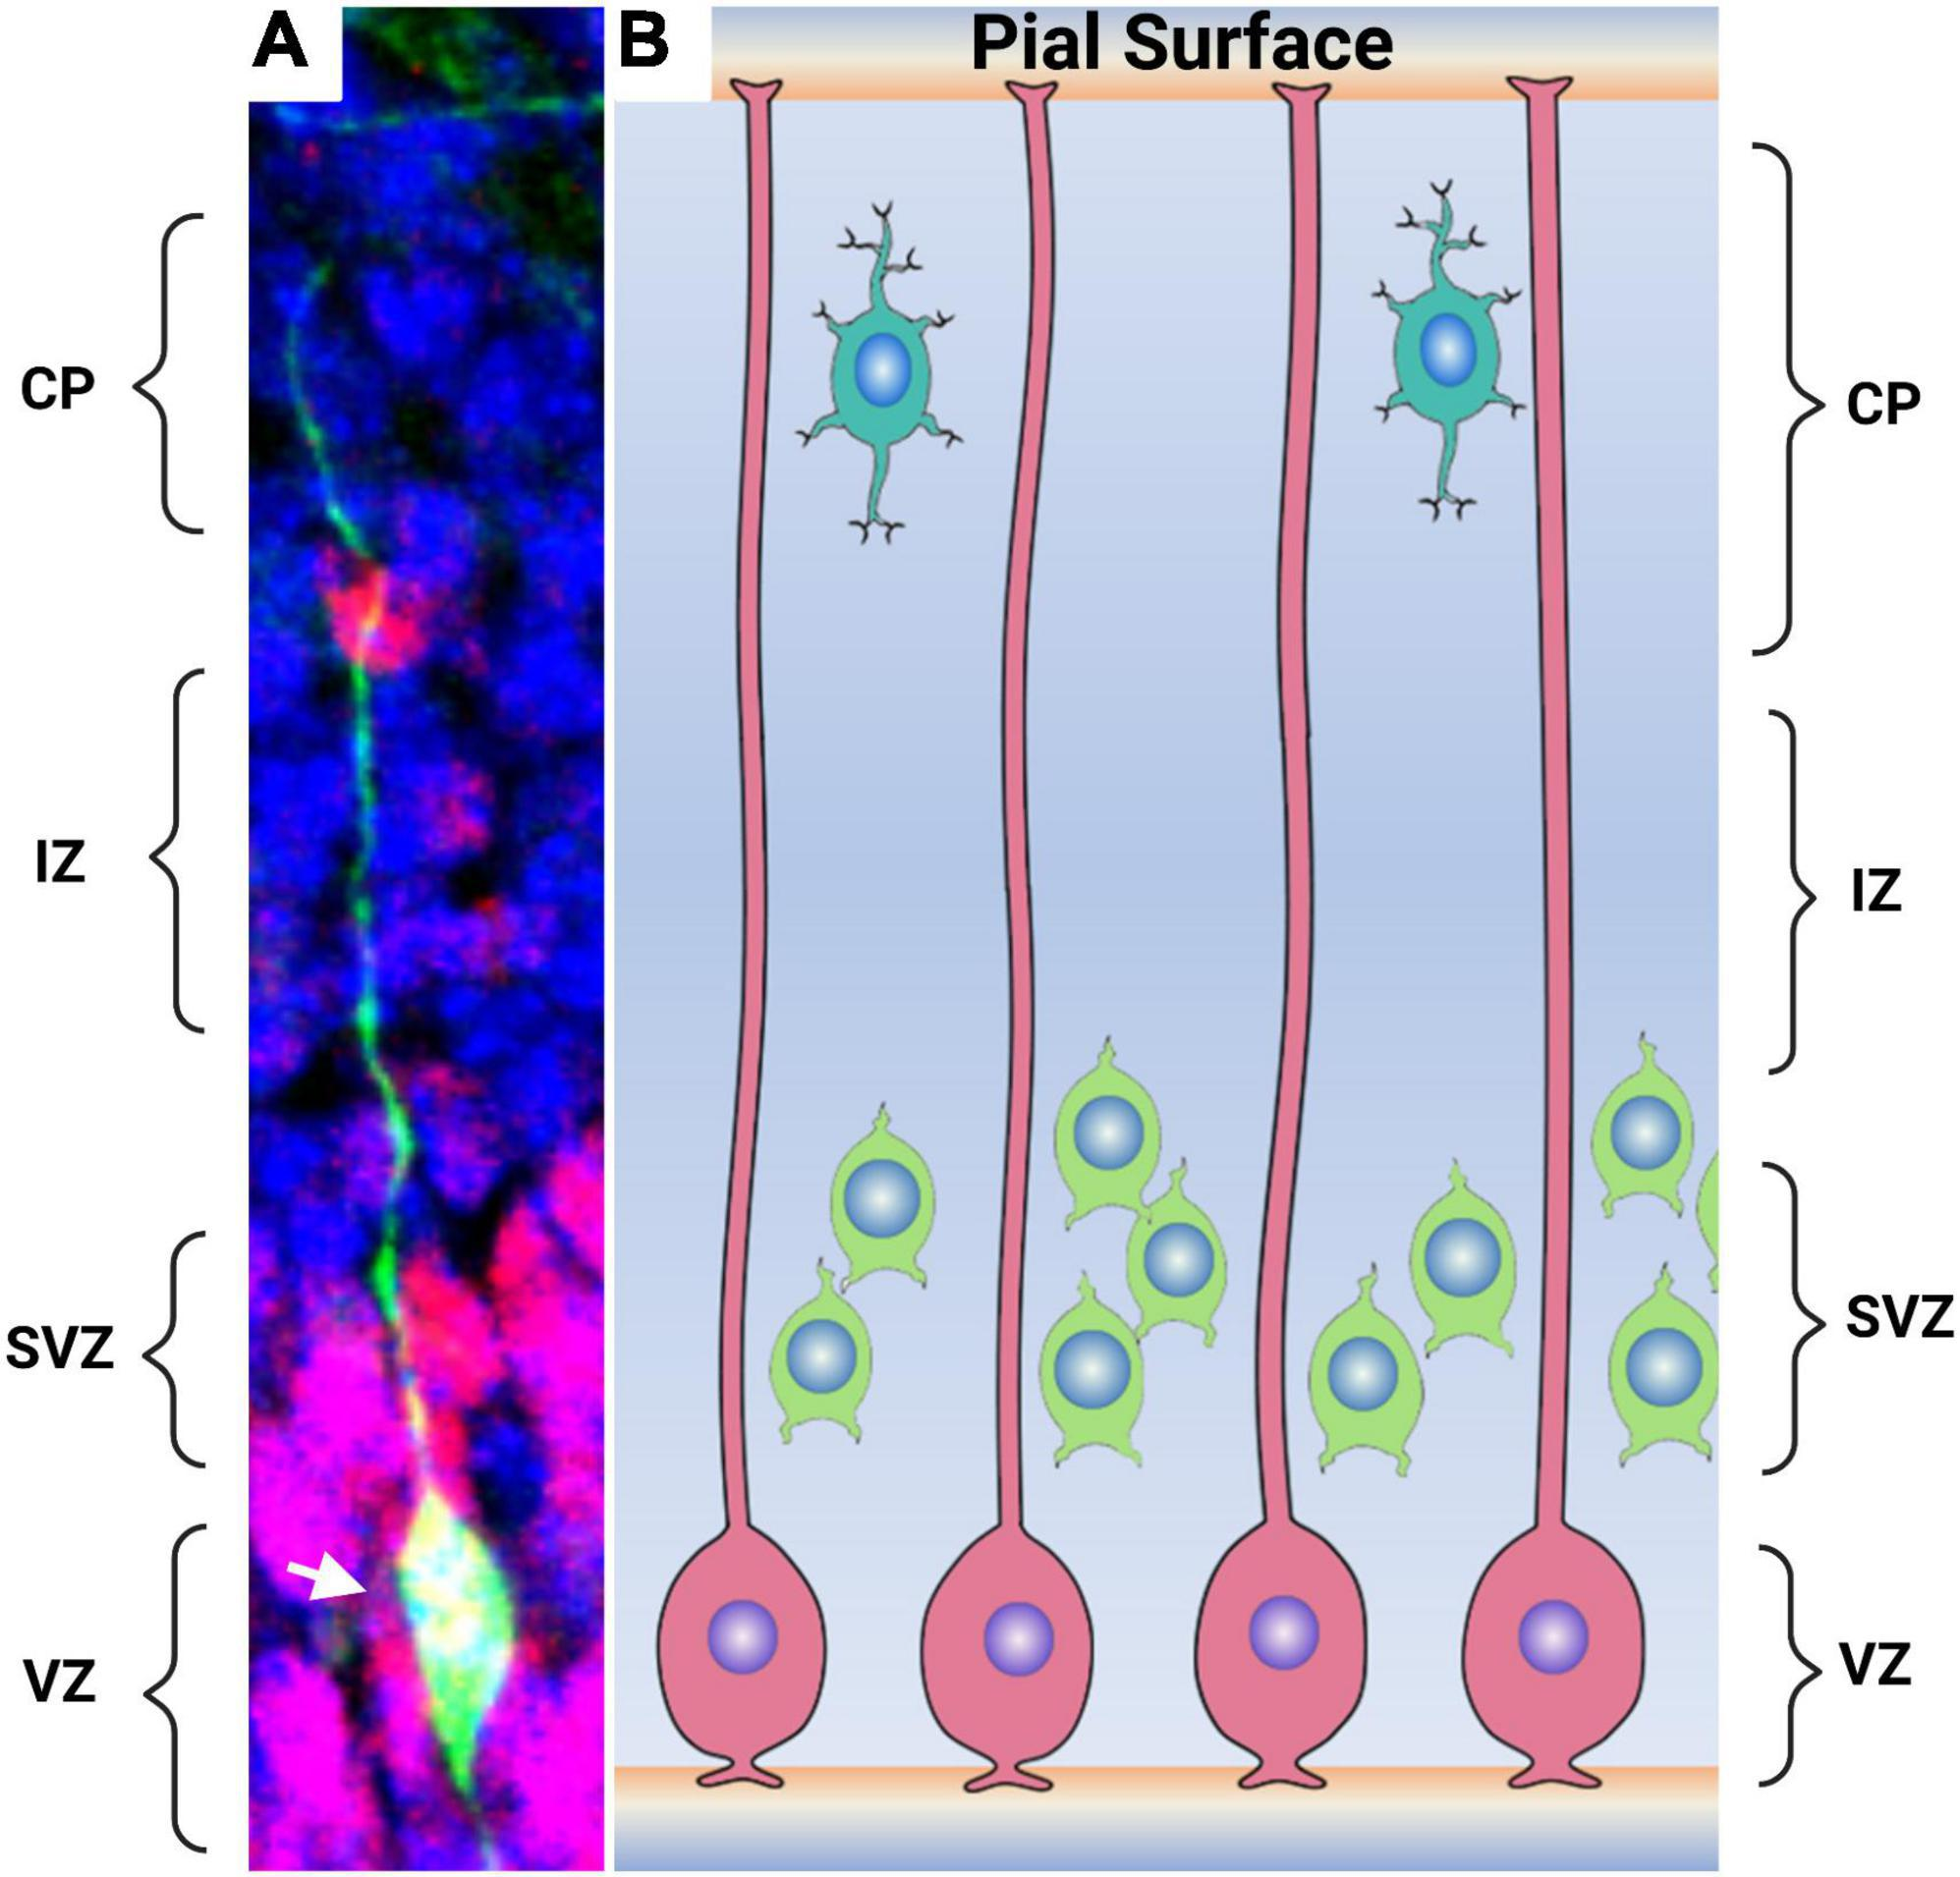
\includegraphics{images/neuro-radialglia.jpg}
\caption{\label{fig:unnamed-chunk-1}As células gliais radiais se prolongam por toda a extensão da parede do tubo neural e são fundamentais para coordenar a migração de diferentes populações celulares durante a histogênese do Sistema Nervoso. VZ: zona ventricular; SVZ zona subventricular; IZ: zona intermediária; CP: placa cortical. \citep{mirandanegrón2022}}
\end{figure}

\hypertarget{cuxe9lulas-de-schwann-e-oligodendruxf3citos}{%
\subsubsection*{Células de Schwann e oligodendrócitos}\label{cuxe9lulas-de-schwann-e-oligodendruxf3citos}}
\addcontentsline{toc}{subsubsection}{Células de Schwann e oligodendrócitos}

Esses tipos celulares são responsáveis por garantir uma condução mais eficiente e célere de impulsos elétricos através dos axônios neuronais por meio da \textbf{mielinização de fibras nervosas}, processo que possibilita a condução saltatória dos potenciais de ação por meio dos nós de Ranvier, pequenos intervalos de membrana desnuda interpostos entre as bainhas de mielina, áreas de revestimento lipídico eletrodinamicamente isolante. Essas células costumam apresentar poucas ramificações (conforme já se pode antever pela própria etimologia grega da palavra ``oligodendrócito''), as quais são primordiais para a fisiologia da mielinização na medida em que se enrolam repetidamente sobre os axolemas neuronais. Nesse âmbito, é necessário destacar que, ao passo que os \textbf{oligodendrócitos} são exclusivos do Sistema Nervoso Central e são capazes de mielinizarem vários axônios ao mesmo tempo, as \textbf{células de Schwann} podem ser observadas exclusivamente no Sistema Nervoso Periférico e podem mielinizar, cada uma, apenas um curto segmento de um dado axônio.

Como resultado desses enrolamentos, essas células gliais formam alguns marcos estruturais idetificáveis por meio da microscopia eletrônica de transmissão e muito úteis para o estudo ultraestrutural das doenças desmielinizantes. Estes correspondem ao \textbf{mesaxônio externo}, uma esprial de \textbf{linhas intraperiódicas} (delimitadas pelo espaço extracelular compreendido entre duas voltas sucessivas do prolongamento mielinizador), uma espiral de \textbf{linhas densas principais} (formadas por uma pequena quantidade de citoplasma dos prolongamentos das células mielinizadoras interposta entre dois folhetos internos da estrutura trilaminar de suas membranas plasmáticas, as quais se encontram quase fundidas) e um \textbf{mesaxônio interno}.

Cabe ressaltar que o processo de mielinização é absurdamente complexo do ponto de vista da Biologia Celular. Resumidamente, seria possível afirmar que, para que a mielina resultante seja viável, são necessárias junções de conexão e de oclusão homotípicas e heterotípicas, proteínas transmembranares responsáveis por compactarem as diversas camadas da espiral formada pelo enrolamento do axônio nos prolongamentos das células mielinizantes (com especial destaque para a proteína zero de mielina e a proteína proteolipídica) e volumes residuais de citoplasma interrompendo a continuidade das linhas densas principais em alguns pontos, correspondendo às \textbf{incisuras de Schmidt-Lantermann}.

Sob a óptica da Neuropatologia, tem-se que as principais doenças que afetam o processo de mielinização decorrem ou de autoimunidades contra proteínas nele envolvidas (como no caso da esclerose múltipla e da Síndrome de Guillain-Barré) ou de mutações nos genes que as codificam. Para se exemplificar esse último cenário, poderíamos pensar na doença de Charcot-Marie-Tooth ligada ao cromossomo X, onde há um defeito molecular na conexina 32 presente nas junções de comunicação homotípicas presentes nas céulas de Schwann, e na doença de Charcot-Marie-Tooth dos tipos 1B e 2, situação na qual anomalias na proteína zero de mielina levam a prejuízos na compactação das bainhas lipídicas formadas pelos prolongamentos mielinizantes.

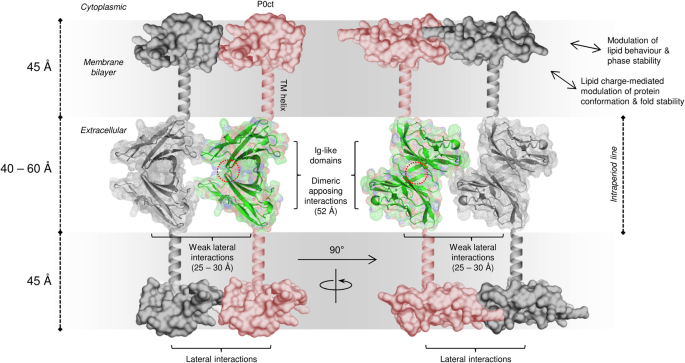
\includegraphics{images/neuro-p0myelin.png}

\hypertarget{cuxe9rebro}{%
\chapter{Cérebro}\label{cuxe9rebro}}

Anatomicamente, o cérebro pode ser considerado, sem sombra de dúvidas, a estrutura mais importante do Sistema Nervoso Central, podendo ser dividido em 47 áreas de Brodmann relacionadas aos mais diversos aspectos da experiência humana, tais como o processamento auditivo central, a empatia, a sensibilidade térmica e dolorosa, a linguagem, a cognição lógico-matemática, a personalidade e a memória. Além disso, temos também inúmeras estruturas subcorticais e diencefálicas vinculadas a mecanismos de analgesia, ao aprendizado motor e ao controle de funções vegetativas.

De uma perspectiva neuroembriológica, tem-se que o cérebro se desenvolve a partir da extremidade cefálica do tubo neural, formada a partir do fechamento do neuróporo rostral durante a quarta semana de desenvolvimento. Esse evento permite a formação de três vesículas encefálicas primárias, as quais correspondem, de rostral a caudalmente, ao \textbf{prosencéfalo}, ao mesencéfalo e ao rombencéfalo. Na quinta semana de desenvolvimento, o prosencéfalo se divide em duas vesículas encefálicas secundárias, correspondentes ao \textbf{telencéfalo}, o qual originará os hemisférios cerebrais, e ao \textbf{diencéfalo}. Deste são oriundas estruturas do:

\begin{itemize}
\tightlist
\item
  \textbf{tálamo}, o grande \emph{relé} sensitivo do Sistema Nervoso.
\item
  \textbf{metatálamo}, onde estão abrigados os corpos geniculados essenciais para as vias visual e auditiva.
\item
  \textbf{epitálamo}, onde se situa a glândula pineal.
\item
  \textbf{hipotálamo}, principal central de controle vegetativo do organismo.
\item
  \textbf{subtálamo}, fundamental para a frenagem de movimentos através da ativação da via indireta dos núcleos da base.
\end{itemize}

Nesse âmbito, é interessante mencionar que a \textbf{protuberância óptica} se desenvolve a partir do diencéfalo na sexta semana de desenvolvimento embrionário, o que justifica a sintopia mantida entre certas estruturas diencefálicas e os nervos ópticos, o quiasma óptico e os tratos ópticos.

No processo de histogênese do prosencéfalo, distinguem-se duas populações celulares primordiais: os \textbf{neuroblastos} e os \textbf{glioblastos}. Enquanto estes darão origem às populações celulares progenitoras dos gliócitos integrantes da macróglia (ou seja, os astroblastos e os oligodendroblastos), aqueles se diferenciarão sequencialmente em neuroblastos bipolares, neurblastos unipolares e neurônios. Vale salientar queé possível que aconteçam interconexões entre os processos de neurogênese e gliogênese, dentre as quais a \textbf{transformação gliogênica} se configura como mecanismo mais comum de conversão de neuroblastos em glioblastos. Finalmente, é preciso ressaltar que, no prosencéfalo, ocorre a migração dos neurônios originados na zona intermediária do tubo neural para a placa cortical, explicando a organização tecidual dos hemisféricos cerebrais num córtex composto por substância cinzenta, onde podem ser visualizados corpos celulares de neurônios, e num centro sensorial composto predominantemente por prolongamentos axônicos de tais neurônios corticais.

No que tange à citoarquitetura dos circuitos neuronais complexos encontrados no córtex cerebral, vale mencionar que esta apresenta variações significativas conforme o grau de desenvolvimento filogenético da espécie estudada e a região cortical analisada. No entanto, é válido afirmar que, para todas as espécies, observa-se uma \textbf{organização laminar} das camadas de células do córtex cerebral, de modo que, usualmente, o córtex se encontra dividido em 6 camadas distintas. Quanto à classificação filogenética dessas regiões cerebrais, vislumbra-se uma subdivisão das áreas corticais em:

\begin{itemize}
\tightlist
\item
  \textbf{arquicórtex}, típico da formação hipocampal.
\item
  \textbf{paleocórtex}, característico do rinencéfalo e de áreas olfativas.
\item
  \textbf{neocórtex}, presente ao longo de 95\% de toda a extensão cortical, correspondendo ao território compreendido pelo isocórtex.
\end{itemize}

Por outro lado, sob uma perspectiva citoarquitetural, o córtex cerebral pode ser classificado como:

\begin{itemize}
\tightlist
\item
  \textbf{isocórtex}, quando estão presentes todas as camadas corticais, que são, de exterior para interior: a camada plexiforme ou molecular, a camada granular externa, a camada das células piramidais, a camada granular interna, a camada ganglionar e a camada das células multiformes.
\item
  \textbf{alocórtex}, no qual ao menos uma das seus camadas supramencionadas se faz ausente.
\end{itemize}

O isocórtex ainda pode ser segmentado em três categorias, o que reflete o alto grau de especialização de diferentes áreas corticais para a efetuação dos mais variados tipos de tarefas e funções. Essas subcategorias são definidas com base no predomínio diferencial de uma camada cortical específica sobre as outras e compreendem as seguintes classificações:

\begin{itemize}
\tightlist
\item
  \textbf{isocórtex homotípico}, encontrado em áreas de associação e caracterizado por possuir estratos de espessuras similares entre si.
\item
  \textbf{isocórtex heterotípico agranular}, observado em áreas motoras primárias e secundárias e organizado de tal maneira que se nota um claro predomínio das camadas compostas por células piramidais sobre os demais estratos corticais.
\item
  \textbf{isocórtex heterotípico granular}, verificado em áreas sensitivas, nas quais existe uma dominância das camadas granulares sobre as outras.
\end{itemize}

Todavia, é preciso ressalvar que a boa visualização dessas camadas corticais e, por conseguinte, a classificação das áreas observadas de acordo com suas características citoarquiteturais e filogenéticas, só podem ser atingidas mediante o emprego de técnicas refinadas de imunofluorescência, as quais possibilitam a marcação dos tipos celulares típicos de cada estrato cortical de acordo com as proteínas expressas especificamente por cada um deles. Nesse contexto, é possível mencionar as seguintes populações celulares para cada lâmina do córtex cerebral:

\begin{itemize}
\tightlist
\item
  \textbf{Camada molecular}: nesse estrato cortical, há o predomínio de \textbf{prolongamentos axonais e dendríticos} de neurônios subjacentes, não sendo possível encontrar uma grande quantidade de células. Entretanto, ocasionalmente se pode deparar com gliócitos e \textbf{células horizontais de Cajal} (também denominadas células de Cajal-Retzius), neurônios glutamatérgicos e \(GABA\)érgicos fundamentais na mediação do processo de corticogênese via secreção de reelina, uma proteína sinalizadora morfogenética.
\end{itemize}

\begin{itemize}
\item
  \textbf{Camada granular externa}: essa camada se encontra composta por densas aglomerações de \textbf{células piramidais} e \textbf{células granulares}. Enquanto estas correspondem a neurônios multipolares do tipo II de Golgi e também são conhecidas como \textbf{células estreladas}, aquelas correspondem a neurônios multipolares do tipo I de Golgi e são os principais tipos de neurônios disparados na ativação do trato corticoespinal e na cognição.
\item
  \textbf{Camada das células piramidais (ou piramidal externa)}: nessa lâmina do córtex cerebral, nota-se um significativo predomínio de \textbf{células piramidais} com pericários de tamanho médio. Vale salientar que, como uma regra geral para essa população celular, observa-se que seus corpos celulares aumentam progressivamente de tamanho conforme mais profundamente se vai adentrando no córtex cerebral. Além dessas células, também se pode encontrar ocasionalmente \textbf{células de Martinotti}, pequenas células poligonais de prolongamentos dendríticos curtos relacionadas à inibição das atividades das células piramidais adjacentes, podendo, dessa maneira, desempenharem funções relevantes no controle motor.
\item
  \textbf{Camada granular interna}: esse estrato do córtex cerebral é constituído primariamente por \textbf{células estreladas} e é tido como a primeira camada cortical a receber aferências talâmicas, sendo, portanto, responsável por retransmiti-las às demais regiões do córtex. Em cortes do giro estriado (área 17 de Brodmann, também conhecida como área visual primária), é possível observar de modo nítido neurônios constituintes da via visual estabelecendo conexões com as células granulares da camada granular interna por meio das \textbf{fibras geniculocalcarinas}, as quais formam a Estria de Gennari, faixa esbranquiçada facilmente reconhecível à examinação macroscópica.
\end{itemize}

\begin{itemize}
\item
  \textbf{Camada granular (ou piramidal interna)}: nessa região do plano estratimérico do córtex cerebral, pode-se visualizar grandes quantidades de \textbf{células piramidais} com somas de dimensões amplas e quantias consideráveis de células estreladas e de Martinotti. No giro pré-central, correspondente à área motora primária, essa camada abriga as \textbf{células de Betz}, os maiores neurônios de todo o Sistema Nervoso e as principais ativadoras de motoneurônios \u03B1 inferiores, estabelecendo sinapses excitatórias glutamatérgicas com estes e projetando-se por meio dos tratos corticoespinais lateral e anterior.
\item
  \textbf{Camada das células multiformes}: apresenta uma gama variada de populações celulares, abrigando células piramidais pequenas, células de Martinotti, células estreladas e \textbf{células fusiformes}. Estas apresentam morfologia alongada, porém, diferentemente das células horizontais de Cajal, dispõem-se perpendicularmente à superfície do córtex cerebral. As células fusiformes encontram-se funcionalmente relacionadas ao envio de impulsos neuronais para outras áreas corticais e para o tálamo.
\end{itemize}

Assim como outras estruturas do neuroeixo, o cérebro se encontra revestido por uma série de folhetos de tecido conjuntivo responsáveis por, dentre outras funções, fornecer proteção mecânica ao tecido nervoso, permitir a nutrição de seus componentes e promover a drenagem sanguínea do encéfalo por meio dos seios venosos. Tais membranas conjuntivas correspondem às meninges e, do ponto de vista estratimérico, elas correspondem, da mais externa para a mais interna, à \textbf{dura-máter}, à \textbf{aracnoide-máter} e à \textbf{pia-máter}.

A dura-máter se encontra aderida ao periósteo dos ossos da calota craniana no encéfalo e forma pregas responsáveis por compartimentalizarem a parte cefálica do paquímero dorsal do corpo, tais como a \textbf{foice do cérebro}, o \textbf{tentório do cerebelo} e a \textbf{foice do cerebelo}. Além disso, essa meninge é composta por um folheto externo e um folheto interno, os quais podem se separar em determinadas regiões para formarem importantes \textbf{seios venosos}, como os seios sigmoides, os seios transversos, o seio sagital superior e o seio sagital inferior, fundamentais para a drenagem venosa do parênquima encefálico.

Internamente à dura-máter, pode-se encontrar a aracnoide-máter, a qual é dividida numa parte mais externa que fica aderida à dura-máter e contribui para a formação de uma camada meníngea protetora espessa (a \textbf{paquimeninge}) e numa parte trabecular que se aprofunda em direção ao \textbf{espaço subaracnoideo}, principal reservatório de líquor cefalorraquidiano no Sistema Nervoso Central. De uma perspectiva histológica, pode-se dizer que a aracnoide-máter é composta fundamentalmente de tecido conjuntivo denso e \textbf{células meningoteliais} revestindo o espaço subaracnoideo.

Ainda mais internamente à aracnoide-máter, pode-se visualizar a pia-máter, o folheto meníngeo \textbf{mais delicado e vascularizado}, que se encontra intimamente aderida ao tecido nervoso e revestida por células meningoteliais de origem embrionária mesenquimatosa. Pelo espaço subaracnoideo transitam artérias dedicadas à irrigação de estruturas cerebrais e esses vasos adentram o parênquima encefálico por meio de canais revestidos por pia-máter e preenchidos por um delgado espaço fisicamente contíguo ao espaço subaracnoideo, denominado espaço perivascular ou \textbf{espaço de Virchow-Robbin}.

\hypertarget{cerebelo}{%
\chapter{Cerebelo}\label{cerebelo}}

De uma perspectiva neuroanatômica, o cerebelo (cuja etimologia latina significa \emph{pequeno cérebro}) corresponde a um órgão do compartimento infratentorial especializado em mecanismos de \textbf{coordenação motora}, \textbf{aprendizado motor} e \textbf{correção dos movimentos corporais}, conectando-se com estruturas tais como o tálamo, o complexo olivar inferior bulbar, o córtex motor, o aparellho vestibular e a medula espinal. Morfologicamente, o cerebelo se situa posteriormente ao quarto ventrículo e se conecta com o tronco encefálico por meio de três pares de pedúnculos cerebelares (superior, médio e inferior), por onde trafegam vias e tratos neuronais responsáveis pelas mais variadas funções desse componente do Sistema Nervoso, que vão desde o planejamento motor junto às áreas 5 e 7 de Brodmann até papéis límicos relacionados à linguagem e à emoção.

Assim como o cérebro, o cerebelo tabmém apresenta uma camada cortical compreendida por substância cinzenta e uma camada medular composta primordialmente por substância branca, as quais correspondem, respectivamente, ao \textbf{córtex cerebelar} e ao \textbf{corpo medular do cerebelo} (denominado também \emph{árvore da vida} por apresentar uma geometria similar àquela observada nos galhos de uma árvore frondosa). Podem ser encontradas esturturas compostas por substância cinzenta mergulhadas no corpo medular, coletivamente referidas como \textbf{núcleos profundos do cerebelo}. Estes abrangem os núcleos \textbf{denteado}, \textbf{interpósito} (formado pela união dos núcleos \textbf{globoso} e \textbf{emboliforme}) e \textbf{fastigial}. Do ponto de vista da divisão longitudinal do cerebelo, cada núcleo se encontra relacionado a funções e vias específicas da motricidade, o que é de grande relevância clínica para a avaliação de quadros de lesões cerebelares no exame físico.

Nesse âmbito, convém salientar que a \textbf{zona verminiana}, composta por uma estrutura altamente segmentada situada ao longo do plano sagital mediano e detentora de um formato parecido com o de uma minhoca (o que justifica seu nome). Essa região se relaciona primariamente com o \textbf{núcleo do fastígio}, estabelecendo conexões com o sistema vestibular por meio da via fastígio-vestibular, essencial para o ajuste de movimentos mediante alterações nas velocidades lineares e angulares do corpo.

Por outro lado, a \textbf{zona paraverminiana}, compreendida por boa parte dos hemisérios cerebelares, relaciona-se ao \textbf{núcleo denteado} e medeia processos vinculados à intercomunicação cérebro-cerebelo para o planejamento motor por intermédio da via eferente dento-tálamo-cortical e da via aferente córtico-ponto-cerebelar.

É necessário apontar que, assim como se pôde perceber para a classificação das regiões do córtex cerebral, o cerebelo também possui uma divisão filogenética, a qual guarda fortes correlações com os aspectos fisiológicos de cada uma de suas regiões. Destarte, é possível subdividir essa estrutura nervosa em:

\begin{itemize}
\tightlist
\item
  \textbf{arquicerebelo}: funcionalmente correlacionado com o vestibulocerebelo e constituído anatomicamente pelo lobo flóculo-nodular.
\item
  \textbf{paleocerebelo}: fisiologicamente relacionado ao espinocerebelo.
\item
  \textbf{neocerebelo}: vinculado ao cerebrocerebelo do ponto de vista funcional.
\end{itemize}

No que diz respeito à anatomia microscópica desse órgão, pode-se afirmar que seu plano estratimérico básico se caracteriza pela presença de uma camada cortical externa de substância cinzenta e uma camada medular interna de substância branca, sendo que o córtex cerebelar pode ser subdividido em três estratos, os quais correspondem, de mais exterior para mais interior, a uma \textbf{camada molecular}, uma camada de \textbf{células de Purkinje} e uma camada de \textbf{células granulosas}.

De modo análogo ao que é observado para a camada molecular do córtex cerebral, a camada molecular cerebelar é relativamente pobre em corpos celulares, porém \textbf{rica em prolongamentos neuronais}. Estes incluem os prolongamentos dendríticos extremamente ramificados das células de Purkinje e os prolongamentos axônicos das células granulosas, os quais se encontram sinapticamente acoplados. Dessa forma, a ativação das células granulares por meio de \textbf{fibras musgosas} provenientes de estruturas extracerebelares promove, consequentemente, a ativação das células de Purkinje. Essa circuitaria neuronal altamente regulada constitui um dos principais aspectos da citoarquitetura cerebelar que possibilitam o aprendizado motor por meio de ativações e silenciamentos sucessivos dos neurônios situados nos núcleos profundos do cerebelo, responsáveis por dispararem as vias eferentes previamente descritas. Dentre as raras populações celulares que possuem seus pericários situados na camada molecular do córtex cerebelar, pode-se elencar as \textbf{células estreladas} e as \textbf{células em cesta}. Estas últimas podem ser classificadas como neurônios multipolares do tipo II de Golgi, configurando-se como células inibitórias \(GABA\)érgicas que promovem a coordenaçãomotora ao inibirem as células de Purkinje e, consequentemente, suprimirem a inibição destas sobre os núcleos cerebelares profundos.

Já a camada de \textbf{células de Purkinje} é composta primariamente por neurônios multipolares do tipo I de Golgi com grandes corpos celulares e uma profusa ramificação dendrítica direcionada para a camada molecular. Essas células são umas das maiores de todo o organismo humano e exercem ação inibitória sobre os neurônios dos núcleos profundos do cerebelo por meio da liberação de \(GABA\) na fenda sináptica compreendida entre essas células ativadoras das vias cerebelares eferentes e os terminais axonais das células de Purkinje. Dessa forma, ocorre um influxo de íons Cl\textsuperscript{-} para o meio intracelular dos neurônios de tais núcleos, hiperpolarizando-os. As células de Pukinje são ativadas principalmente por meio da ação das \textbf{fibras trepadeiras}, que se originam do \textbf{núcleo olivar inferior} e emitem prolongamentos axônicos que parecem se entrelaçar helicoidalmente ao redor das fibras nervosas representadas pelos axônios das células de Purkinje, de modo similar ao que é constatado para as plantas epífitas, que parecem se enrolar ao redor dos troncos das árvores com as quais estabelecem relações ecológicas desarmônicas.

Por fim, cabe salientar que a \textbf{camada granulosa} do córtex cerebelar é composta primordialmente por \textbf{células granulosas}, neurônios multipolares do tipo Golgi I que emitem extensos prolongamentos axônicos retilíneos e amielínicos para a camada molecular do córtex cerebelar, e \textbf{células de Golgi}, as quais correspondem a interneurônios inibitórios \(GABA\)érgicos ativados pelas fibras musgosas e responsáveis por suprimirem as atividades das células granulosas. Teoriza-se que o papel das células de Golgi no contexto das intrincada circuitaria neural cerebelar esteja voltado à \textbf{plasticidade neuronal} no córtex cerebelar e ao rearranjo espaço-temporal dos níveis de atividade das células granulosas e de suas conexões sinápticas.

\hypertarget{plexo-coroide}{%
\chapter{Plexo Coroide}\label{plexo-coroide}}

Sob uma óptica histológica, pode-se asserir que a população celular mais representativa das regiões nas quais se faz presente o plexo coroide corresponde às \textbf{células ependimárias}, embriologicamente derivadas das células ventriculares que povoam a zona ventricular do tubo neural durante o processo de histogênese do tecido nervoso. Além de tais células, também é possível encontrar \textbf{tanicitos} em algumas regiões específicas do sistema ventricular encefálico, os quais correspondem a células derivadas da glia radial bipolar detentoras de uma morfologia intermediária entre os astrócitos e as células ependimárias. Dessa forma, é válido frisar que as células ependimárias e os tanicitos constituem os principais componentes neuroepiteliais do epêndima, imprescindível para a produção e a movimentação do líquido cefalorraquidiano.

Como já se pode inferir a partir das populações celulares gliocíticas descritas acima, o plexo coroide (ou corioide) corresponde a uma associação de \textbf{estruturas circumventriculares} e um \textbf{epêndima} de características epitelioides que abriga células especializadas na produção do líquor a partir do plasma sanguíneo. Nesse sentido, é pertinente lembrar que os chamados \emph{órgãos circumventriculares} são regiões do Sistema Nervoso Central nas quais se observam descontinuidades da barreira hematoencefálica e, dessa forma, representam áreas de fluxo de substâncias facilitado entre o meio intravascular e o tecido nervoso. Do ponto de vista ultraestrutural, o plexo coroide constitui-se essencialmente pela interface entre uma rede de capilares fenestrados com diafragma situada no interior de uma massa de tecido conjuntivo frouxo e o epêndima sobrejacente.

Assim, pode-se dizer que o plexo coroide está presente nas paredes do terceiro e do quarto ventrículos, onde uma película fina de \textbf{pia-máter} altamente vascularizada denominada \textbf{tela coroide} oferece o aporte sanguíneo necessário para a produção de líquor e, nas fissuras coroides dos ventrículos laterais, situadas nas seções mediais desses componentes do sistema ventricular encefálico, entre o fórnice e o tálamo. Nessas regiões verifica-se, além da intensa produção de líquor, um incisivo e perene \textbf{monitoramento imunológico} por parte de macrófagos, linfócitos e células dendríticas encontradas no tecido conjuntivo frouxo que sustenta o plexo coroide.

Ultraestruturalmente, as células ependimárias apresentam grandes quantidades de \textbf{mitocôndrias} e múltiplas \textbf{invaginações basais} de seus domínios de membrana basolaterais, fatores que as caracterizam como células detentoras de intensa atividade metabólica e elevadas taxas de transporte ativo ocorrendo por bombas proteicas incrustadas na membrana plasmática. Ademais, a presneça de \textbf{microvilosidades} e eventuais \textbf{cílios} em seus domínios de membrana apicais é significativa do ponto de vista histofisiológico, haja vista que as células em questão também efetuam a absorção e a circulação do líquor. Finalmente, é interessante apontar a existência de uma resistente \textbf{barreira hematoliquórica} constituída por junções de oclusão e interdigitações estabelecidas entre células ependimárias adjacentes. Tais especializações laterias de membrana são, pois, fundamentais para se evitar a passagem direta de moléculas do sangue para o líquido cefalorraquidiano.

\hypertarget{medula-espinal}{%
\chapter{Medula Espinal}\label{medula-espinal}}

De uma perspectiva neuroanatômica, a medula espinal se constitui como um grande \textbf{\emph{conduit} neuronal} central responsável por integrar o encéfalo com os compontnes do Sistema Nervoso Periférico. Isso possibilita, por exemplo, que o núcleo rubro medeie o controle ultrapreciso da musculatura intrínseca da mão por meio do trato rubroespinal, e que o sistema límbico receba e processe informações aferentes de dor crônica captadas por fibras nociceptivas amielínicas do tipo C na periferia do corpo e transmitidas ao prosencéfalo pro meio da \textbf{via paleoespinotalâmica}.

Convém, entretanto, frisar que as características fisiológicas da medula espinal vão muito além do que aquelas que se poderia esperar de um simples cilindro constituído puramente por prolongamentos axônicos responsáveis por carregarem \emph{inputs} oriundos dos tecidos periféricos e \emph{outputs} para estes dirigidos. Desse modo, verifica-se que a medula espinal também está envolvida no controle das funções vegetativas do organismo por meio dos \textbf{núcleos intermédio-laterais} toracolombares e dos \textbf{núcleos intermédio-mediais} sacrais, em mecanismos de analgesia mediados pela \textbf{Substãncia Gelatinosa de Rolando} e até mesmo em arcos reflexos altamente intrincados, com a ativação e a inibição de grupamentos musculares inteiros. Nesse âmbito, é interessante ressaltar que o fenômeno da modulação negativa da dor por meio de estímulos táteis, explicado pela \textbf{Teoria da Comporta da Dor}, ocorre ao nível da medula espinal e hodiernamente é alvo de múltiplos estudos que visam à invenção de novos tratamentos farmacológicos da dor crônica.

Macroscopicamente, a medula espinal apresenta como limite superior a \textbf{decussação das pirâmides} e como limite inferior o \textbf{ligamento coccígeo}, originado a partir da parte dural do \textbf{filamento terminal}, emitido a partir do \textbf{cone medular}. A medula espinal apresenta uma organização metamérica, que, no entanto, é díspar daquela observada para a coluna vertebral, estojo ósseo que delimita a parte caudal do paquímero dorsal e abriga a estrutura nervosa em questão. Isso se dá em decorrência das taxas de crescimento diferenciais observadas para essas duas estruturas durante o processo de organogênese, de tal forma que é válido afirmar que um determinado segmento vertebral abriga estruturas nervosas referentes ao metâmero espinal dois níveis inferiores a ele. Assim, na seção do canal vertebral compreendida pela vértebra T\(V\), é possível encontrar o segmento medular T7.

Diferentemente do que se verifica para o encéfalo, a medula apresenta uma estratimeria na qual a \textbf{substância branca} composta majoritariamente por células da glia e prolongamentos axônicos ascendentes e descendentes se encontram na \textbf{periferia} do tubo e a \textbf{substância cinzenta}, compreendida por gliócitos e corpos celulares de neurônios, encontra-se numa posição \textbf{central}. Isso se dá naturalmente mediante o processo de histogênese do órgão em questão, o qual se desenvolve a partir do tubo neural, cujo lúmen se oblitera quase completamente nesse processo. É interessante apontar que a divisão clássica da substância cinzenta do \emph{H} medular num \textbf{corno ventral eferente motor} e um \textbf{corno dorsal aferente sensitivo} possui fundamentação embriológica. Ao passo que este é oriundo de uma estrutura denominada \textbf{placa alar}, a qual se forma por meio das células constituintes da parede dorsal do tubo neural e se diferencia em estruturas nervosas sensitivas por meio da ação do morfógeno \(Wnt\), aquele é originado a partir da \textbf{placa basal}, que se desenvolve a partir da parede ventral do tubo neural e se diferencia em neurônios motores inferiores através da indução morfogenética efetuada pela proteína \(SHH\) em suas células. Nesse sentido, pode-se lembrar que, diferentemente do que se observa na medula de um indivíduo que já completou seu desenvolvimento embrionário, a medula primitiva apresenta sulcos laterais responsáveis por demarcar o limite entre as placas alares e as placas basais, denominados \textbf{sulcos limitantes}.

Outro aspecto anatômico no qual se pode notar claras diferenças entre as organizações macroscópicas e mesoscópicas do encéfalo e da medula espinal se dá na organização dos folhetos meníngeos, uma vez que, na medula, a dura-máter não se encontra aderida ao periósteo das vértebras, apresentando-se relativamente solta no interior do canal vertebral, formando o \textbf{saco dural}, uma estrutura fibrosa de \textbf{tecido conjuntivo denso} responsável por fornecer proteção mecânica à medula. Externamente ao saco dural, é possível observar a presença de tecido conjuntivo frouxo, tecido adiposo unnilocular e elementos neurovasculares preenchendo o \textbf{espaço epidural}. Vale salientar que, dentre as estruturas vasculares que podem ser encontradas nessa região, tem-se o \textbf{plexo venoso de Batson}, o qual promove a drenagem sanguínea da medula espinal e se conecta com veias das cavidades torácica e abdominopélvica. Tais conexões explicam o porquê de certos tipos de neoplasias, como o câncer de próstata, efetuarem metástases hematogênicas parao Sistema Nervoso Central.

Microscopicamente, é possível subdividir a substância cinzenta da medula espinal, que se dispõe num formato parecido com uma letra \emph{H} ou com uma borboleta (ganhando, por isso, a denominação de \emph{H} medular), em uma série de \textbf{lâminas} ou \textbf{núcleos} conhecidos como \textbf{lâminas de Rexed}. Cada uma dessas lâminas desempenha papéis específicos na modulação das atividades dos tratos espinais que trafegam pela substância branca e nas funções motoras e sensitivas desempenhadas pelo neuroeixo em sua interface de integração com o restante do organismo por meio do Sistema Nervoso Periférico. É interessante ressaltar que a proporção entre as áreas ocupadas pela substância cinzenta e pela substância branca aumenta craniocaudalmente, de forma que a medula espinal sacral possui um predomínio de substância cinzenta e a medula espinal cervical, de substância branca.

\hypertarget{nervos}{%
\chapter{Nervos}\label{nervos}}

A partir de uma óptica neuroanatômico, é válido afirmar que os nervos são as principais estruturas que compõem o \textbf{Sistema Nervoso Periférico} e, por isso, funcionam como \emph{fios} que abrigam importantes circuitos neuronais responsáveis pela comunicação entre o Sistema Nervoso Central e as demais regiões do corpo. Isso possibilita que o Sistema Nervoso como um todo atue, ao lado do Sistema Endócrino, como uma rede de integração entre os múltiplos órgãos das várias regiões do corpo.

Ao todo, possuímos \textbf{12 pares de nervos cranianos} e \textbf{31 pares de nervos espinais}. Enquanto estes se originam a partir da substância cinzenta do \emph{H} medular, aqueles se originam de núcleos imersos na substância branca do \textbf{tronco encefálico}, a exemplo do nervo vago (NC X), o qual se origina parcialmente do núcleo dorsal motor do nervo vago, e do nervo oculomotor (NC III), que possui seu componente autonômico oriundo do núcleo de Edinger-Westphal, ou de \textbf{projeções telencefálicas} e \textbf{diencefálicas}, como se observa para o nervo olfatório (NC I) e o nervo óptico (NC II), respectivamente.

De forma geral, pode-se dizer que todo nervo possui um componente \textbf{aferente sensitivo} e um componente \textbf{eferente motor} e, do ponto de vista histológico, compõe-se por conjuntos de prolongamentos axônicos revestidos por membranas protetivas de tecido conjuntivo e fibras colágenas. Tais prolongamentos podem ou não estar mielinizados e isso dependerá da atividade das \textbf{células de Schwann}, os principais gliócitos do Sistema Nervoso Periférico. Essas células apresentam \textbf{núcleos sinuosos e alongados} que parecem acompanhar as trajetórias percorridas pelos prolongamentos nervosos.

Os nervos usualmente podem ser encontrados em estreita associação com elementos vasculares tais como as veias de médio calibre e as artérias musculares constituintes dos \textbf{feixes vásculo-nervosos}, e se encontram compartimentalizados em \textbf{feixes} e \textbf{fascículos} nervosos por meio das membranas conjuntivas supramencionadas. Estas correspondem ao \textbf{epineuro}, ao \textbf{perineuro} e ao \textbf{endoneuro}.

Nesse âmbito, é possível mencionar que, enquanto o \textbf{epineuro} une vários fascículos nervosos em um só nervo e é composto primordialmente por \textbf{tecido conjuntivo denso}, o \textbf{perineuro} delimita os fascículos nervosos e corresponde a uma bainha conjuntiva constituída por uma série de fibroblastos modificados com formato achatado entremeados por fibras colágenas. Existe ainda o \textbf{endoneuro}, que corresponde a uma delicada película de \textbf{tecido conjuntivo frouxo} que reveste fibras nervosas individuais.

Entre os fascículos nervosos, pode-se observar, no interior das bainhas conjuntivas supradescritas, \textbf{vasos sanguíneos} responsáveis pela vascularização do tecido nervoso periférico. Vale salientar que os nervos configuram-se como estruturas de notável relevância clínica no exame físico neurológico, podendo ser lesados por uma miríade de afecções com as mais variadas etiologias, como a hanseníase, a neuropatia diabética e a esclerose múltipla.

\hypertarget{guxe2nglios}{%
\chapter{Gânglios}\label{guxe2nglios}}

\hypertarget{guxe2nglios-sensitivos}{%
\section{Gânglios Sensitivos}\label{guxe2nglios-sensitivos}}

As fibras sensitivas constituintes dos nervos espinais apresentam seus somas situados em dilatações localizadas na \textbf{raiz dorsal} de seus nervos, em estruturas conhecidas como \textbf{gânglios sensitivos das raízes dorsais}. Esses neurônios pseudounipolares transmitem informações sensitivas ao Sistema Nervoso Central por meio das vias \textbf{coluna dorsal-lemnisco medial}, responsável pela condução de informações relacionadas ao tato epicrítico, à sensibilidade vibratória e à propriocepção consciente de todo o corpo com exceção da cabeça e do pescoço, e \textbf{anterolateral}, a qual conduz informações relacionadas ao tato protopático, à propriocepção inconsciente, à nocicepção e à termocepção.

Como característica histológica peculiar dos gânglios sensitivos, é possível mencionar a presença de gliócitos especializados, denominados \textbf{células satélites}, ``contornando'' e sustentando os corpos celulares e os neuritos dos neurônios sensitivos. Ao emitirem um prolongamento centrípeto em direção à medula espinal e um prolongamento centrífugo em direção à periferia do organismo, os gânglios sensitivos proporcionam a integração somatossensorial entre diferentes regiões do corpo, o que é de especial importância para a defesa do organismo e para a mediação de \textbf{arcos reflexos}.

\hypertarget{guxe2nglios-autonuxf4micos}{%
\section{Gânglios Autonômicos}\label{guxe2nglios-autonuxf4micos}}

Essas estruturas integram a \textbf{divisão visceral} do Sistema Nervoso e são fundamentais para o controle das funções vegetaticas, estabelecendo conexões com os gânglios pré-vertebrais simpáticos, os gânglios das cadeias paravertebrais e os núcleos intermédio-mediais da medula espinal. Nesse sentido, vale salientar que, nas lâminas observadas, verifica-se a presença dessas estruturas no \textbf{Sistema Nervoso Entérico}, onde formam o \textbf{plexo mioentérico} (ou de \textbf{Auerbach}), situado entre as camadas musculares circular interna e longitudinal externa do intestino e envolvido na regulação da motilidade destas, e o \textbf{plexo submucoso} (ou de \textbf{Meissner}), localizado na camada submucosa e essencial para o controle da motilidade do estrato muscular da mucosa e para o controle quimioceptivo e mecanoceptivo da peristalse.

Ainda se pode vislumbrar a presneça de pequenos gânglios autonômicos em meio ao tecido conjuntivo presente nas trabéculas da \textbf{glãndula submandibular}, onde medeia suas atividades secretórias conectando-se com fibras provenientes do nervo facial.

\hypertarget{aplicauxe7uxe3o-cluxednica}{%
\section{Aplicação Clínica}\label{aplicauxe7uxe3o-cluxednica}}

O vírus causador da \emph{Herpes zoster} tende a se alojar nos gânglios sensitivos das raízes dorsais dos nervos espinais quando se converte em seu estado latente após uma primoinfecção. Assim, mediante episódios de imunossupressão intensa, esse patógeno pode voltar à sua forma ativa e proporcionar o aparecimento de feridas máculo-papulares e vesiculares que se distribuem metamericamente na superfície do corpo, obedecendo os padrões de delimitação dos \textbf{dermátomos}. Cabe ressaltar que essas lesões podem ser desencadeadas por estresse emocional severo e podem ulcerar se deixadas sem tratamento, o que favorece a ocorrência de infecções secundárias.

\hypertarget{mecanorreceptores}{%
\chapter{Mecanorreceptores}\label{mecanorreceptores}}

\hypertarget{corpuxfasculos-de-vater-paccini}{%
\section{Corpúsculos de Vater-Paccini}\label{corpuxfasculos-de-vater-paccini}}

Os corpúsculos de Vater-Paccini correspondem a estruturas nervosas encapsuladas por \textbf{lamelas concêntricas} de tecido conjuntivo e responsáveis pela detecção de informações relacionadas à \textbf{sensibilidade vibratória} e à \textbf{pressão} exercida em \textbf{camadas profundas} da derme reticular e na hipoderme, onde tais estruturas componentes do Sistema Somatossensorial são mais numerosas. Por possuírem um complexo revestimento de fibras colágenas entremeadas por fluido intersticial, esses receptores são sensíveis até mesmo às mais sutis variações da pressão aplicada sobre a superfície da pele, encontrando-se distribuídos em abundância por regiões do tegumento recobertas por pele espessa e sujeitas a atritos e forças friccionais intensas e constantes, a exemplo da palma da mão e da superfície plantar do pé.

Convém, todavia, salientar que essas terminações nervosas mecanorreceptoras não são exclusivas do Sistema Tegumentar, podendo também ser visualizadas em vísceras secretoras como o \textbf{pâncreas}, em \textbf{articulações} e no \textbf{periósteo} que reveste os componentes ósseos do esqueleto. Não se sabe ao certo os papéis fisiológicos efetuados pelos corpúsculos de Vater-Paccini nestes locais, especialmente no que concerne à população desses mecanorreceptores encontrada nas trabéculas conjuntivas do pâncreas. Entretanto, é teorizado que eles possam estar envolvidos no controle central da secreção realizada por essa importante glândula anfícrina retroperitoneal por meio da detecção de variações na pressão hidrostática no interior dos ductos secretores ao decorrer da ejeção do suco pancreático para a porção descendente do duodeno.

De um ponto de vista neurofisiológico, é possível afirmar que as informações captadas pelos corpúsculos de Paccini chegam ao \textbf{córtex somatossensorial primário}, correspondente ao \textbf{giro pós-central} (áreas 1, 2 e 3 de Brodmann), por meio da via \textbf{coluna dorsal-lemnisco medial}. Nesse âmbito, observa-se que o primeiro neurônio da via, cuja terminação nervosa periférica forma o corpúsculo de Paccini, possui seu pericário situado nos \textbf{gânglios sensitivos das raízes dorsais} dos nervos espinais e, ao adentrar na medula, envia um longo prolongamento axônico para o \textbf{tálamo} por meio do \textbf{funículo posterior} da substância branca medular. Particularmente, verifica-se que há um expressivo direcionamento das fibras nervosas para núcleos talâmicos responsáveis pela retransmissão das informações referentes à sensibilidade vibratória, à propriocepção consciente e ao tato epicrítico, merecendo destaque os núcleos \textbf{ventral póstero-lateral} e \textbf{ventral póstero-medial}.

Ao chegar nesses centros talâmicos, o impulso nervoso é retransmitido para a \textbf{camada IV (granular interna)} do córtex somatossensorial primário, onde obedece um padrão de distribuição \textbf{somatotópico}

\hypertarget{botuxf5es-gustativos}{%
\chapter{Botões Gustativos}\label{botuxf5es-gustativos}}

Histologicamente, essas \textbf{estruturas neuroepiteliais} formam pequenos aglomerados elipsoides de células incrustadas no epitélio pavimentoso estratificado não-queratinizado característico da mucosa de revestimento especializada da língua, podendo ser encontrados nas superfícies das papilas \textbf{fungiformes}, \textbf{foliáceas} e \textbf{circunvaladas} (a exceção são as papilas filiformes, que cumprem funções mais relacionadas à fricção do alimento com a superfície lingual do que à sensibilidade espacial gustatória). Nessas estruturas neuroepiteliais, é possível distinguir a existência de três populações celulares:

\begin{itemize}
\item
  As células \textbf{basais}, que funcionam como células-tronco e se encontram destinadas à reposição contínua das células gustativas.
\item
  Já as \textbf{células gustativas} são especializadas na detecção de sabores por meio do reconhecimento de moléculas solúveis dispersas na saliva e se degradam muito rapidamente quando comparadas a outras populações celulares, haja vista suas meias-vidas estimadas de 5 a 10 dias. Cabe ressaltar que essas células são providas de abundantes microvilos apicais que usualmente dispõem de grandes quantidades de receptores metebotrópicos dedicados à percepção dos sabores liberados pela comida e à transdução de sinais elétricos por estes proporcionados.
\end{itemize}

\begin{itemize}
\tightlist
\item
  Por fim, as \textbf{células sustentaculares} são responsáveis pela sustentação das populações celulares supramencionadas, atuando como um componente estromal dos botões gustativos.
\end{itemize}

Nesse âmbito, também é válido mencionar que as células gustativas receptoras se encontram divididas em \textbf{3 subtipos} principais, cada qual dedicado à percepção de diferentes modalidades gustativas. Assim, tem-se que, ao passo que as células gustativas do \textbf{tipo I} se encontram especializadas na captação de informações relativas ao sabor salgado, as células gustativas do \textbf{tipo II} estão voltadas à detecção do doce, do \emph{umami} (sabor característico de alimentos ricos em glutamato, tais como o peixe cru, os cogumelos e alguns tipos de queijo) e do amargo por meio de receptores metabotrópicos denominados \textbf{transducinas}. Finalmente, tem-se que as células gustatórias do \textbf{tipo III} possuem propriedades características de células excitáveis, sendo capazes de conduzir potenciais de ação e desempenharem respostas elétricas vinculadas aos sabores azedo e salgado por intermédio de despolarizações proporcionadas pela entrada de cátions (Na\textsuperscript{+} e Ca\textsuperscript{2+}) através de canais iônicos voltagem-dependentes situados nos polos apicais de tais células.

Quando as moléculas responsáveis pela percepção do sabor se dissolvem na saliva e adentram nos \textbf{poros gustativos}, pequenas aberturas por meio das quais o domínio de membrana apical das células gustativas se abre na cavidade oral, ocorre, portanto, o disparo de cascatas de sinalização intracelulares responsáveis por promoverem a \textbf{exocitose de ATP} para a região de contato entre o botão gustativo e ramos nervosos especiais dos nervos facial (NC VII), vago (NC X) e glossofaríngeo (NC IX). Dessa forma, mediante a ativação dessas estruturas nervosas, a informação gustativa é carreada até o \textbf{córtex gustativo primário}, localizado nos giros da ínsula posteriores, por meio de uma trajetória nervosa que passa pelo \textbf{núcleo do trato solitário (NTS)}.

\hypertarget{drogas-de-abuso}{%
\chapter{Drogas de Abuso}\label{drogas-de-abuso}}

Do ponto de vista do Código Penal Brasileiro, as drogas de abuso podem ser classificadas em lícitas (a exemplo do álcool e da nicotina, substâncias que apresentam alto potencial dependogênico em função da comercialização disseminada e da maior aceitação social para com sua utilização, que pregressamente era vista até mesmo como distintivo de \emph{status} econômico) e ilícitas (grupo que inclui a maconha, o ácido lisérgico, as anfetaminas, o MDMA, o \emph{skank}, os inalantes, as \emph{club drugs} e inúmeras outras substâncias que constituem problemas de saúde pública de proporções geopolíticas ao se considerar o impasse do tráfico internacional de drogas e o surgimento de extensas cenas de uso intinerantes que moldam o cenário das grandes metrópoles, como a \emph{Cracolândia} paulistana e a \emph{Skid Row} em Los Angeles). Vla salientar que inúmeras substâncias originalmente planejadas como fármacos passaram a apresentar um caráter de droga de abuso como consequência de fenômenos relacionados à medicalização da vida moderna e à automedicação, haja vista a incidência crescente de síndromes de abstinência ocasionadas pela retirada de benzodiazepínicos e drogas-Z em indivíduos que realizavam uso cotidiano desses medicamentos para dormir. Nesse sentido, tem-se observado que, seguindo as recomendações de agências reguladoras como a \emph{CDC}, muitos entes federados estadunidenses vêm aplicando restrições cada vez mais duras sobre a distruibuição e a fabricação de opioides potentes como o fentanil, o qual, embora possa apresentar um emprego muito valioso na forma de adesivos transdérmicos para o manejo da dor em pacientes em Cuidados Paliativos, tem contribuído para a epidemia de abuso de opioides que assola o país desde o final da década de 90. Sob o ponto de vista farmacodinâmico, pode-se categorizar as drogas de abuso de acordo com suas principais ações sobre os sistemas de neurotransmissão, embora devemos sempre ter em mente que, mesmo dentre as drogas de uma determinada categoria, existe grande heterogeneidade quanto a seus mecanismos de ação, os quais nem sempre são muito bem entendidos. Assim, seria possível traçar a seguinte classificação para as drogas de abuso:

\begin{itemize}
\item
  \textbf{Álcool:} presente em diferentes títulos em diferentes bebidas destiladas ou fermentadas, como o uísque, a cerveja, o rum, o saquê, o corote, a cachaça e o vinho.
\item
  \textbf{Nicotina:} agonista total de receptores ionotrópicos de acetilcolina, primeiramente extraída da planta \emph{Nicotiana tabacum}, pode ser encontrada em cigarros, charutos, essências para narguilês e nos \emph{e-líquidos} utilizados em \emph{vapes} (cigarros eletrônicos).
\item
  \textbf{Derivados da maconha:} incluem o \emph{skank}, uma espécie de ``maconha sintética'' e o haxixe, um exsudato resinoso extraído das glândulas presentes nos tricomas do terço superior de plantas femininas da espécie \emph{Cannabis sativa}. Seus efeitos sobre o sistema de recompensa e outras áreas do córtex cerebral se dão pelas substâncias tetrahidrocanabidiol (THC), relacionado à euforia e às alucinações relatadas durante o uso, e canabidiol, amplamente pesquisado em razão de seus efeitos terapêuticos putativos para quadros de epilepsia, êmese induzida por medicamentos e doenças neurodegenerativas.
\item
  \textbf{Hipnóticos e Sedativos:} destacam-se nesse grupo substâncias corriqueiramente utilizadas como fármacos, como o clonazepam (um benzodiazepínico), o zolpidem (um hipnótico muito potente) e o fenobarbital (barbitúrico utilizado para tratamento de epilepsias refratárias). Compartilham o mecanismo de ação comum de atuarem como moduladores alostéricos positivos de receptores \(GABA_A\),assim como o álcool, sendo que quadros de intoxicação por essas substâncias podem levar ao óbito por parada respiratória na medida em que ocorre supressão importante de centros vegetativos bulbares, o que pode ser revertido com o uso do antídoto flumazenil.
\item
  \textbf{Opioides:} essa classe farmacológica foi um marco na história da Anestesiologia e compreende uma série de alcaloides naturais extraídos da papoula ( \emph{Papaver somniferum} ), como a morfina, a codeína e a tebaína, e opioides sintéticos fabricados por meio da introdução ou da modificação de grupos funcionais dessas substâncias, a exemplo da heroína, da petidina, do fentanil, do tramadol e da metadona. Atuam em receptores opioides \(\mu\), \(\delta\) e \(\kappa\) promovendo modulação da dor e inibição de interneurônios \(GABA_B\) responsáveis por regularem a atividade da via mesolímbica, deixando-a hiperativa.
\item
  \textbf{Estimulantes:} englobam substâncias como as anfetaminas, a cocaína, o metilfenidato, a atomoxetina e a efedrina, as quais atuam promovendo extravasamento de neurotransmissores excitatórios - especialmente a norepinefrina e a dopamina - de suas vesículas sinápticas, promovendo também o acúmulo destes no meio extracelular por meio de uma inversão na dinâmica de recaptação e transporte de proteínas de armazenamento vesicular como a \(VMAT\) e de recaptação de neurotransmissores, como a \(NET\), as quais passam a atuar como bombas de extrusão de neurotransmissores para o meio externo. Para o tratamento dos sintomas das crises de abstinência provocados pela retirada do uso dessas substâncias, podem ser empregados antipsicóticos e \(\beta\)-bloqueadores.
\item
  \textbf{Alucinógenos:} abrigam um amplo rol de substâncias, muitas das quais são utilizadas como enteógenos por comunidades tradicionais e não possuem mecanismos de ação muito bem conhecidos. Nesse sentido, podemos citar como representantes dessa classe o ácido lisérgico (LSD), a psilocibina, a mescalina, o MDMA, o DMT (dimetiltriptamina) e os alcaloides \(\beta\)-carbolínicos encontrados na \emph{ayahuasca}, na harmala e no cipó-mariri.
\end{itemize}

No que diz respeito às manifestações clínicas e aos sintomas das síndromes de abstinência relativas ao uso de cada uma das classes supramencionadas de drogas de abuso, pode-se dizer que estas são extremamente variadas e, em última instância, dependem não só de mecanismos de \emph{up-regulation} ou \emph{down-regulation} de receptores nas membranas neuronais como também de modificações ainda desconhecidas sobre os sistemas de neurotransmissão e neuromodulação. A mesma heterogeneidade pode ser verificada quanto às sensações relatadas mediante o uso dessas substâncias, uma vez que elas diferem significativamente entre si quanto a seus alvos de ação. Dessa forma, noticia-se:

\begin{itemize}
\item
  \textbf{Álcool:} constitui a droga de abuso mais consumida atualmente e atua como modulador alostérico positivo de receptores \(GABA_A\), facilitando a ligação do ácido \(\gamma\)-aminobutírico a esse canal iônico operado por ligantes, proporcionando um influxo de íons \(Cl^-\) que hiperpolariza a célula, fazendo com que seja mais difícil dela ser disparada. Nesse sentido, pequenas doses de álcool podem proporcionar euforia e comportamento social desinibido na medida em que neurônios de centros superiores responsáveis pela regulação do comportamento são inibidos. Entretanto, à medida que a alcoolemia aumenta (e, por apresentar uma cinética de eliminação de ordem zero, os níveis plasmáticos de etanol costumam variar erraticamente e serem de difícil controle em situações de intoxicação), essa inibição neuronal pode se disseminar para os núcleos da base, o cerebelo e o hipocampo, levando ao aparecimento de ataxia, descoordenação da marcha e amnésia anterógrada (a qual, a nível molecular, pode estar relacionada a subtipos de receptores neuronais que contêm uma subunidade \(\alpha_5\)).
\item
  \textbf{Nicotina:} conforme postula Stephen Stahl, esse agonista total de receptores nicotínicos possui um potencial dependogênico estimado em 32\% e atua no Sistema Nervoso Central ativando receptores nicotínicos e promovendo despolarização neuronal, que causa uma sensação de relaxamento e despertar. Em função de sua via de administração se dar pelo fumo (via inalatória), esses efeitos são observados de modo extremamente rápido. Acredita-se que sua atuação em receptores nicotínicos dos subtipos \((\alpha_7)_5\) e \((\alpha_4)_2(\beta_2)_3\) esteja envolvida nos aspectos psicológicos subjacentes a seu uso e à sua dependência.
\item
  \textbf{Maconha e seus derivados:} ao atuarem em receptores canabinoides do tipo \(CB_1\) distribuídos por grandes extensões do Sistema Nervoso Central de modo análogo a canabinoides endógenos derivados do ácido araquidônico, como a anandamida, o tetrahidrocanabinol (THC) e o canabidiol regulam a atividade de liberação de neurotransmissores por meio de terminais nervosos pré-sinápticos. Em baixas doses, isso parece se relacionar a sensações de relaxamento, tranquilidade e bem-estar, porém, se os níveis dessas substâncias se elevarem, o indivíduo poderá relatar crises psicóticas e alucinações. Vale ressaltar que as substâncias presentes na maconha podem provocar, mediante uso crônico, embotamento afetivo, dificuldades para dormir e em funções sociais, perda da personalidade e de habilidades, além de transtornos psicóticos. Isso é particularmente grave em adolescentes, uma vez que a organização citoarquitetural de suas vias de comunicação encefálicas ainda não se encontra completamente madura e a maconha parece promover proliferação sináptica desordenada, prejudicando o desenvolvimento neuropsicocognitivo.
\item
  \textbf{Opioides:} além de atuar de modo similar às dinorfinas e endorfinas produzidas endogenamente durante situações estressantes a partir da clivagem da pré-opiomelanocortina e, por conseguinte, proporcionarem uma intensa analgesiaatuando em receptores na medula e na substância cinzenta periaquedutal, os opioides também parecem ativar a via mesolímbica dando uma sensação de ``barato'' ao se ligarem a receptores expressos em neurônios \(GABA\)érgicos moduladores dessa via e diminuir a ativação destes. Assim, ao fazer uso de um opioide potente como o fentanil, um indivíduo pode relatar uma sensação de prazer, relaxamento e bem-estar com cessação de suas dores, efeitos que podem ser seguidos de sonolência. No entanto, em quadros de intoxicação por opioides, os quais podem ser tratados com o uso do antagonista opioide naltrexona em sua forma inalável, é comum que o indivíduo apresente miose, xerostomia, cólicas e prurido. Vale ressaltar, no entanto, que para o tratamento da abstinência por retirada de opioide, recomenda-se utilizar a metadona, um opioide menos potente cuja meia-vida de eliminação longa impede a ocorrência de variações bruscas dos níveis das drogas em uso.
\item
  \textbf{Sedativos e Hipnóticos:} como mencionado anteriormente, ao se utilizar um barbitúrico, um benzodiazepínico ou uma droga-Z e as moléculas desses fármacos ocuparem seus sítios alostéricos nos receptores \(GABA_A\) (localizados nas regiões de transição entre as subunidades \(\alpha\) e \(\gamma\) desse canal iônico operado por ligantes), ocorre uma mudança conformacional nesse receptor que favorece a ligação das moléculas de \(GABA\) (ácido \(\gamma\)-aminobutírico) a seus dois sítios ortostéricos situados na transição entre as subunidades \(\alpha\) e \(\beta\) dessas proteínas. Desse modo, nota-se uma inibição intensa da atividade neuronal, o que, embora seja benéfico para situações como o controle do estado de mal epiléptico (quadro para o qual se costuma administrar uma dose de ataque de 10 miligramas de diazepam intravenoso), pode levar à amnésia anterógrada, ataxia, marcha ebriosa, depressão respiratória e óbito, especialmente se esses medicamentos forem ingeridos junto com o álcool, que também atua potencializando a transmissão \(GABA\)érgica (vale lembrar que é exatamente esse o princípio da ``boa noite Cinderela'', droga de estupro que leva flunitrazolam em sua composição). Entretanto, em doses menores, essas drogas tendem a provocar sentimentos de tranquilidade intensa, relaxamento, sonolência e hipotonia muscular.
\item
  \textbf{Estimulantes:} em vista de seus mecanismos de ação se centrarem na liberação neurotransmissores excitatórios para o meio extracelular, potencializando a ação destes sobre as sinapses, pode-se elencar como os principais efeitos agudos decorrentes do uso de drogas como a cocaína, a atomoxetina, o metilfenidato, a anfepramona (muito utilizado por caminhoneiros que realizam longas viagens noturnas) e a efedrina sensações de euforia e hipervigilância, acompanhadas de tendências maníaca, alerta extremo, palpitações, tremores, diaforese e midríase (percebe-se que alguns desses sintomas, especialmente aqueles que se manifestam a nível físico, encontram-se relacionados à hiperativação simpática). Essas substâncias possuem alto potencial de causarem dependência e a síndrome de abstinência por sua retirada é marcada por anedonia, desejo intenso de dormir intercalado por períodos de agitação e \emph{craving} pela droga, os quais podem ser tratados por meio de \(\beta\)-bloqueadores, fármacos que atuarão controlando os sintomas físicos supramencionados, e antipsicóticos. A tendência de indivíduos que fazem uso de estimulantes do SNC é de que, com o passar do tempo e com o desenvolvimento de tolerância às drogas menos potentes, eles busquem drogas capazes de promover a liberação de monoaminas de modo mais intenso.
\item
  \textbf{Alucinógenos:} de um pondo de vista farmacodinâmico, os mecanismos de ação dessas drogas são variados, complexos e ainda incompreendidos, porém em grande parte estes parecem estar relacionados ao estado de humor do indivíduo que as consome, podendo seus efeitos serem fortemente influenciados por este. Dessa maneira, as alucinações visuais, auditivas, cenestésicas, olfativas e gustatórias apresentadas por pessoas que fazem uso de substâncias como o ácido lisérgico podem ser caracterizadas como \emph{good trips}, nas quais o indivíduo se sente espiritualmente elevado e iluminado por forças divinas, ou \emph{bad trips}, nas quais o usuário da droga - que provavelmente já se encontrava ansioso ou deprimido antes do consumo da substância - relata viver um verdadeiro pesadelo acordado, ouvindo vozes aterrorizantes e enxergando monstros. Ademais, um fenômeno pouco compreendido que pode ser causado por essas drogas são os \emph{flashbacks}, períodos nos quais os indivíduos que já as utilizaram experienciam reviver seus momentos de contato com a substância. Em virtude de provocarem uma tolerância brusca e intensa, é raríssimo observar quadros de dependência para essa classe de drogas de abuso.
\end{itemize}

De modo geral, os mecanismos fisiopatológicos subjacentes ao desenvolvimento de transtornos de dependência química e abuso de substâncias se relacionam à hiperativação da via mesolímbica cerebral (cuja hiperativação de seus neurônios dopaminérgicos também pode ser vista em transtornos psicóticos, explicando os sintomas positivos da esquizofrenia), uma espécie de sistema de recompensa endógeno é disparado toda vez que participamos de atividades prazerosas como forma de promover aprendizado de padrões de comportamento repetidos. Neuroanatomicamente, a via mesolímbica tem início nos núcleos da área tegmentar ventral do mesencéfalo, os quais se projetam para o núcleo \emph{accumbens}, na base do telencéfalo, que projeta eferências para áreas terciárias situadas primordialmente no córtex pré-frontal, embora estas também possam se dirigir para a amígdala e para o hipocampo, o que é fundamental para se compreender a importância de fatores socioafetivos na patogênese da dependência química e a relevância das memórias relativas ao uso da substância para possíveis quadros de recaída. Inicialmente, o indivíduo dependente (que, muito mais do que uma simples predisposição genética, usualmente sofre de solidão, isolamento social e tristeza profunda), passa buscar a substância (não só a droga, como também comportamentos de risco, como jogos de azar) como forma de se livrar de suas angústias e a sensação de ``barato'' proporcionada pela ativação forçada da via mesolímbica funciona como reforço positivo para que esse sujeito recorra novamente à droga no futuro. Entretanto, a via mesolímbica se adapta rapidamente à neurotransmissão modificada em consequência do uso da droga, ocorrendo dessensibilização de seus neurônios por modificações covalentes de seus receptores \(D_2\) ou ainda internalização destes em vesículas citoplasmáticas, de forma que passa a ser necessária uma dose muito maior da droga para se alcançar o mesmo efeito inicial, levando ao desenvolvimento da tolerância. Cabe ressaltar que as adaptações moleculares efetuadas pelos neurônios em resposta ao uso da droga podem fazer com que o indivíduo se sinta agitado, indisposto ou depressivo na ausência da substância, quando as condições de neurotransmissão forem restituídas a seus estados basais. Assim, o indivíduo passa a sofrer de um quadro de abstinência mediante a retirada da droga, o qual se caracteriza por desejo intenso de consumir a substância para se livrar dos sintomas físicos desconfortáveis causados por sua ausência, de forma que o reforço positivo representado pelo ``barato'' por esta provocado durante a fase inicial do processo de dependência é suplantada por um reforço negativo. Como curiosidade, vale mencionar que temos vias neurais específicas encarregadas por ``frear'' a atividade da via mesolímbica, muitas das quais se iniciam no córtex pré-frontal dorsolateral (DLPFC), região cuja densidade neuronal se encontra diminuída em indivíduos que sofrem de dependência química.

Vale salientar que os sintomas reportados na síndrome de abstinência por álcool (esse mesmo mecanimso também se aplicaria a outros moduladores alostéricos positivos de receptores \(GABA_A\), como os benzodiazepínicos, os barbitúricos e as drogas-Z), como o famoso \emph{delirium tremens}, podem ser explicados com base no fato de que, diante de uma situação de inibição prolongada causada por uma hiperpolarização decorrente da atividade aumentada de receptores \(GABA_A\), os neurônios do Sistema Nervoso Central passam a internalizar tais receptores inibitórios em vesículas citoplasmáticas e expressar maiores quantidades de receptores glutamatérgicos \(NMDA\) em seus terminais pós-sinápticos na tentativa de sofrerem maior excitação. No entanto, quando o álcool sai de cena e a neurotransmissão é reconstituída a seus estados pregressos, esses neurônios passam a ficar hiperexcitáveis, explicando, por exemplo, o tremor e a agitação da abstinência alcóolica.

Em se tratando do tratamento farmacológico dos transtornos de abuso de álcool e nicotina, condições que, de acordo com o \(III\) Levantamento Nacional sobre o Uso de Drogas pela População Brasileira (FIOCRUZ), afetam, respectivamente, 2,3 e 4,8 milhões de pessoas em todo o território nacional, é possível destacar as seguintes estratégias farmacológicas:

\textbf{Para o tratamento do transtorno de dependência de álcool:}

\begin{itemize}
\item
  \textbf{Naltrexona:} esse análogo sintético da oximorfina atua como ANTAGONISTA de receptores opioides, eliminando o prazer relacionado ao consumo do álcool ao modular a atividade de neurônios da via mesolímbica por mecanismos ainda pouco conhecidos.
\item
  \textbf{Acamprosato:} fármaco relativamente caro, pode ser utilizado para o tratamento do \emph{craving} pelo álcool bem como para o manejo de sintomas de abstinência, dado que atua como ANTAGONISTA de receptores glutamatérgicos do tipo \(NMDA\).
\item
  \textbf{Benzodiazepínicos:} podem ser administrados em pacientes que dão entrada em serviços de urgência apresentando tremores, ansiedade e agitação excessivos desencadeados por abstinência ao álcool, uma vez que atuarão como MODULADORES ALOSTÉRICOS POSITIVOS de receptores \(GABA_A\), facilitando a neurotransmissão inibitória.
\item
  \textbf{Dissulfiram:} comercializado com os nomes ``Antabuse'' e ``Antietanol'', esse fármaco atua como INIBIDOR IRREVERSÍVEL da enzima aldeído-desidrogenase, responsável por converter o acetaldeído, metabólito tóxico oriundo da biotransformação do etanol pela enzima álcool-desidrogenase, em acetato. Desse modo, toda vez que o paciente que faz uso de dissulfiram ingere álcool, ele passará a apresentar quadros de diarreia e vômito em decorrência do acúmulo de acetaldeído, o que constitui um reforço negativo para que ocorra interrupção do uso da substância. Ademais, por mecanismos até então não conhecidos (ou não revleados para o público geral), o dissulfiram também é capaz de provocar disgeusia toda vez que o paciente ingere álcool.
\end{itemize}

Cabe ressaltar que, para o tratamento de sintomas referentes à síndrome de abstinência alcóolica, o paciente também pode efetuar uso crônico de \textbf{antiepilépticos} como o topiramato, o valproato e a carbamazepina e de \textbf{antidepressivos tricíclicos} como a imipramina, que inibe os sistemas de recaptura de monoaminas, especialmente a norepinefrina, a serotonina e a dopamina, ou de \textbf{inibidores seletivos da recaptação de serotonina}, tais como a fluoxetina e a sertralina.

\textbf{Para o tratamento do transtorno de dependência de nicotina:}

\begin{itemize}
\item
  \textbf{Terapia de reposição de nicotina:} tem como objetivo auxiliar na cessação do hábito de fumar e auxiliar no manejo da abstinência nicotínica ao fornecer níveis plasmáticos de nicotina sustentados para a ativação de receptores nicotínicos espalhados pelo Sistema Nervoso Central, apresentando a vantagem de reduzir o consumo de substâncias carcinogênicas presentes no tabaco. A nicotina utilizada para esse propósito pode ser encontrada em inúmeras apresentações farmacêuticas, como chicletes, gomas, \emph{sprays} nasais, adesivos transdérmicos e pastilhas.
\item
  \textbf{Bupropiona:} corresponde a um antidepressivo atípico que atua como INIBIDOR DA RECAPTAÇÃO DE NOREPINEFRINA E DOPAMINA e ANTAGONISTA de receptores nicotínicos. É um exemplo de pró-fármaco, uma vez que são seus metabólitos treo-hidrobupropiona e eritro-hidrobupropiona que exercem o efeito sobre os alvos farmacológicos. Acredita-se que possam atuar na via mesolímbica ao interferirem na transmissão dopaminérgica.
\item
  \textbf{Vareniclina:} princípio ativo dos medicamentos ``Champix'' e ``Chantix'', a vareniclina age como AGONISTA total de receptores nicotínicos \((\alpha_7)_5\) e agonista parcial de receptores nicotínicos dos subtipos \((\alpha_4)_2(\beta_2)_3\), \((\alpha_4)_3(\beta_2)_2\) e \((\alpha_3)_m(\beta_4)_n\). Além disso, por mecanismos até então não explicados, é capaz de proporcionar o aparecimento de um gosto desagradável na boca, similar ao de esterco, quando o indivíduo faz uso do cigarro.
\end{itemize}

Cabe destacar que, apesar de apresentarem considerável eficiência, serem de grande valia no âmbito clínico e oferecerem estratégias invadoras para o tratamento de afecções multifatoriais de natureza extremamente complexa (a exemplo de uma vacina não-proteica para a nicotina, que atualmente se encontra na fase \(III\) de seus estudos clínicos), as abordagens farmacológicas para o tratamento de transtornos de dependência devem vir sempre acompanhadas de medidas não-farmacológicas primordiais para o sucesso terapêutico, como a psicoterapia e a modificação dos hábitos de vida (deixar de frequentar cenas de uso da substância, por exemplo). Nesse sentido, convém destacar que organizações como os Alcóolicos e Narcóticos Anônimos (e, mais recentemente, os Jogadores Anônimos) podem se mostrar muito úteis para o acolhimento empático de pacientes que sofrem dos transtornos supramencionados, os quais em grande parte foram intensificados por uma rede de apoio inexistente ou fragilizada.

Brevemente, a partir de referências conceituadas como o livro ``Psicofarmacologia'' de Stephen Stahl, é possível traçar as seguintes definições para os seguintes termos:

\begin{itemize}
\item
  \textbf{Uso abusivo de drogas:} refere-se a um padrão na utilização de substâncias biologicamente ativas (as drogas, que, por definição, abrangem os fármacos) para fins recreativos ou de performance (como tem sido cada vez mais evidenciado no contexto universitário pelo uso de metilfenidato), sem finalidades terapêuticas.
\item
  \textbf{Adição:} diz respeito a padrões comportamentais e psicológicos de uso abusivo de substâncias, no qual o indivíduo adito apresenta envolvimento emocional com a droga em decorrência de suas experiências pessoais vividas enquanto se encontrava sob a influência desta, não sendo raro que ele fique anedônico e experiencie fissura ( \emph{craving} ) intenso pela substância mediante a interrupção de seu uso.
\item
  \textbf{Dependência:} caracteriza o estado de adaptações fisiológicas produzido pela administração repetida de determinadas substâncias, o qual se mostra patente mediante a retirada desta, haja vista que tais modificações fisiológicas levam ao aparecimento de sintomas físicos de abstinência.
\item
  \textbf{Tolerância:} a tolerância a uma determinada droga é observada quando, após administração repetida desta, tornam-se necessárias doses cada vez maiores para se atingir o mesmo efeito tecidual inicial. Isso é um grande problema para algumas das grandes classes de psicofármacos mais utilizadas no cenário farmacoepidemiológico hodierno, como os benzodiazepínicos e as drogas-Z.
\end{itemize}

  \bibliography{book.bib,packages.bib}

\end{document}
